%---PACKAGES----------------------------------------
\documentclass[a4paper,10pt]{article}

\usepackage{import}
\import{Packages/}{custom_packages.tex}
\import{Packages/}{custom_macros.tex}

\title{\textbf{Notes on Quiver Gauge Theories}}
\author{Louan Mol\\ \textit{Université Libre de Bruxelles}}
\date{}

% DOCUMENT -----------------------------

\begin{document}

\begin{titlepage}
    
    \maketitle

    \thispagestyle{empty}

    \vspace{2cm}

    \begin{abstract}
        These notes are meant as a work support. The goal is to reproduce and regroup the basics of quiver gauge theories. 
    \end{abstract}

    \vfill

    \hfill Last updated on \today.
    
\end{titlepage}
  
\pagebreak

\tableofcontents

\pagebreak

\nocite{*}

\section{The brane-world paradigm}

    We consider our world to be a slice in the ten-dimensional spacetime of type II superstring theory, i.e. the worldvolume of a D$3$-brane. More precisely, we consider a stack of $N$ D$3$-branes in order to have a $\U(N)$ gauge group. The spacetime is therefore not necessarily $\R^{1,9}$ but of the more general form
    \begin{equation*}
        M = \R^{1,3}\times M^{(6)}.
    \end{equation*}
    This is the so-called \emph{brane-world paradigm}. In particular, we will be interested in type IIB string theory because of its self-duality under S-duality\marker.
    
    Independently from string theory, we ask to have $\mN=1$ supersymmetry for the $4$-dimensional worldvolume theory. This constrains the transverse space $M^{(6)}$ to be compact, complex, Kähler and to have $\SU(3)$ holonomy, see appendix \ref{sec:appCY}. Namely, $M^{(6)}$ must be a Calabi-Yau threefold.
    
    If we let the worldvolume of the D$3$-branes carry the requisite gauge theory while the bulk contains gravity, we can relax the compactness condition and study non-compact threefolds. In other words, $M^{(6)}$ is taken to be an affine variety that localy models a Calabi-Yau threefold. Intuitively, this can be understood as a Kaluza-Klein compactification where we take the size of the compact dimensions to infinity. The four-dimensional gravity coupling constant being inversely proportional to this quantity, there is no gravity in this limit. This makes the analysis much simpler and therefore also serves as an argument to ignore gravity in the worldvolume theory. Thus far, we have $n$ D$3$-branes on which there is a $\U(N)$ gauge group and transverse to which gravity propagates.

    The only smooth Calabi-Yau threefold is $\C^3$ so we are lead to consider singular Calabi-Yau manifolds or, more precisely, Calabi-Yau orbifolds. We usually denote $S\equiv M^{(6)}$ to remind us of the singular aspect. String theory being a theory of extended objects, it is well-defined on such singularities. We will see that this singular structure of the geometry will break $\U(N)$ into products of gauge groups.
    
    From the point of view of the orbifold, the D$3$-brane is a point. Consequently, there is a crucial relationship between the D$3$-brane worldvolume theory and the Calabi-Yau singularity: the former parametrizes the latter. In other words, the classical vacuum of the gauge theory should be, in explicit coordinates, the defining equation of $S$.

    Mathematically, this brane-world paradigm is the realization of branes as supports of vector bundles (sheaf). Gauge theories on branes are intimately related to algebraic constructions of stable bundles, i.e. holomorphic or algebraic vector bundles that are stable in the sense of geometric invariant theory. In particular, D-brane gauge theories manifest as a natural description of symplectic quotients and their resolutions in geometric invariant theory.

    To summarize in more mathematical terms, our D-branes, together with the stable vector bundle (sheaf) supported thereupon, resolves the transverse Calabi-Yau orbifold which is the vacuum for the gauge theory on the worldvolume as a GIT quotient \marker.

    \begin{result}
        We consider $N$ D$3$-branes carrying a $\U(N)$ gauge group on various orbifolds of $\R^6$. Requiring $\mN=1$ supersymmetry for the worldvolume theory imposes that the transverse space must be a Calabi-Yau orbifold. Ignoring gravity for the worldvolume theory and if we want more interresting cases, we can actually consider the larger class of non-compact singular Calabi-Yau spaces.
    \end{result}
    

\section{The simplest case: $S=\C^3$}

    \subsection{Generalities}

        Let us by studying the simplest configuration were the transverse Calabi-Yau space is non-singular, i.e. it is a proper smooth Calabi-Yau threefold. The only smooth Calabi-Yau threefold is $S=\C^3$. In this case, the spacetime is simply flat space $\R^{1,9}=\R^{1,3}\times\R^6$ with a choice a complex structure on $\R^6$. As mentioned above, the worldvolume theory has a $\U(N)$ gauge group. Type IIB superstring theory is a ten-dimensional $\mN=2$ theory so it has $32$ supercharges. The presence of the branes breaks the Lorentz symmetry of $\R^{1,9}$ as
        \begin{equation}
            \SO(1,9)\to\SO(1,3)\times\SO(6),
        \end{equation}
        whereby breaking half of the supersymmetries, see appendix \ref{sec:appCY}. We are thus left with $16$ supercharges. In four dimensions, this corresponds to $\mN=4$. The worldvolume theory for $S=\C^3$ is therefore $D=4,\mN=4$ $\U(n)$ SCFT gauge theory. This worldvolume theory, obtained in the non-singular case $S=\C^3$, is called the \emph{parent theory}.

        Note that the D$3$-brane will warp the flat space metric to that of $AdS_5\times S^5$ and the bulk geometry is not strictly $\C^3$. However, as stated above, we are only concerned with the local gauge theory and not with gravitational back-reaction, therefore it suffices to consider $S$ as $\C^3$.

    \subsection{Matter content}

        As discussed in appendix \ref{sec:N4SCFT}, there is only one $D=4,\mN=4$ SCFT theory, up to a choice of gauge group $G$. In our case, $G=\U(N)$. The isometry group of the transverse space $\R^6$ is $\SO(6)\cong\SU(4)$. It is a global symmetry of the field theory since the field living on the branes are to be interpreted as its tranverse oscillations. These global symmetries of worldvolume theory lead to the R-symmetry group $\SU(4)_R$. The only $\mN=4$ supermutliplet can be rewritten in terms of $\mN=1$ supermultiplets as follows:
        \begin{equation}
            [\mN = 4 \text{ vector multiplet}] : V = (\lambda_\alpha, A_\mu, D) \oplus \Phi_A = (\phi^A,\psi^A_\alpha,F^A).
        \end{equation}
        with $A=1,2,3$. In other words, after removing the auxiliary fields, the matter content is
        \begin{itemize}
            \item a $\U(N)$ gauge field $A_\mu$ which transforms as a singlets under $\SU(4)_R$:
            \begin{align}
                \text{Gauge transformation} &: A_\mu\mapsto UA_\mu U^{-1}+U\p_\mu U^{-1},\qquad U\in\U(N)\label{eq:transfA1}\\
                \text{R-symmetry} &: A_\mu\mapsto A_\mu.\label{eq:transfA2}
            \end{align}
            \item $4$ Weyl fermions $\psi^{a}_\alpha\equiv(\lambda_\alpha,\psi^1_\alpha,\psi^2_\alpha,\psi^3_\alpha,)$ that transform under the adjoint of $\U(N)$ and are mixed together under the representation $\boldsymbol{4}$ of $\SU(4)_R$. This means that each fermion $\psi^a$ takes values in $\mathfrak{u}(N)$ and we denote the components by $\psi^a_{IJ}$ ($I,J=1,\dots,N$). Explicitely:
            \begin{align}
                \text{Gauge transformation} &: \psi^a \mapsto U \psi^a U^\dagger ,\qquad U\in\U(N),\label{eq:transfpsi1}\\
                \text{R-symmetry} &: \psi^a\mapsto R\indices{^a_b}\psi^b,\qquad R\in\SU(4)_R.\label{eq:transfpsi2}
            \end{align}
            Note that this gives us $4N^2$ Weyl fermions in total.
            \item $3$ complex scalar fields $\phi^A$ transforming under the adjoint representation of $\U(N)$ and under the two-times anti-symmettric representation of $\SU(4)_R$. This means that each $\phi^A$ takes values in $\mathfrak{u}(N)$ and we denote the components by $\phi^A_{IJ}$. Recall that $\SU(4)\cong\SO(6)$ so the action of the R-symmetry can be seen as the $\boldsymbol{3}$ of $\SU(3)\subset\SU(4)_R$ acting on three complex scalars $\phi^1$ or equivalently as the $\boldsymbol{6}$ of $\SO(6)_R$ acting on $6$ real scalars $X^m$, the real and imaginary parts of the $\phi^A$. They are interpreted as the oscillations of the branes in the transverse space. Explicitely:
            \begin{align}
                \text{Gauge transformation} &: X^m \mapsto U X^m U^\dagger ,\qquad U\in\U(N),\label{eq:transfphi1}\\
                \text{R-symmetry} &: X^m \mapsto R\indices{^m_n}X^n,\qquad R\in\SO(6)_R.\label{eq:transfphi2}
            \end{align}
            Note that this gives $6N^2$ real scalars in total. They are the superpartners of the fermions\marker.
        \end{itemize}
        Note that the gauge group $\U(N)$ can also be seen as the group of isometries the metric space $\C^N$ to itself, i.e. $\Hom(\C^N,C^N)$. From this point of view, the transformations \eqref{eq:transfA1}-\eqref{eq:transfphi2}can be summarized as
        \begin{align}
            A_\mu&\in\Hom(\C^N,\C^N),\label{eq:AHom}\\
            \psi&\in\boldsymbol{4}\otimes\Hom(\C^N,\C^N),\label{eq:psiHom}\\
            X&\in\boldsymbol{6}\otimes\Hom(\C^N,\C^N).\label{eq:phiHom}
        \end{align}

\section{Projection to daughter theories}

    \subsection{Generalities}

        When the transverse space is singular, the worldvolume theory corresponds to a specific projection of the parent theory that we found in the smooth case $S=\C^3$. We call it the \emph{daughter theory}. This projections depends on the type of singularity that one considers.

        We now wish to pick a discrete group $\Gamma$ and which acts non-trivially on $\R^6$. There are several possibilities:
        \begin{itemize}
            \item $\Gamma\subset\SU(4)$ naturally acts on $\R^6$. This does not require a choice of complex structure. We get an $\mN=0$ theory.
            \item $\Gamma\subset\SU(3)$ naturally acts on $\C^3$, this also requires a choice of complex structure on $\R^6$. We get an $\mN=1$ theory.
            \item $\Gamma\subset\SU(2)$ naturally acts on the second factor of $\C\times\C^2$, so this requires a choice of complex structure on $\R^6$. We get an $\mN=2$ theory.
        \end{itemize}

        For now, we are interested with $\mN=1$ theories so we consider $\Gamma\subset\SU(3)$ with the action
        \begin{equation}
            \cdot:\left(
            \begin{array}{ccc}
                \Gamma\times\C^3 & \longrightarrow & \C^3 \\
                (\gamma,z) & \longmapsto & \gamma\cdot z
            \end{array}
            \right)
        \end{equation}
        is the representation of $\Gamma$ coming from the fundamental representation of $\SU(3)$, so $\cdot$ is just the matrix product. We can see that the origin is always a fixed point so this action is never free. Since $\C^3$ is a smooth manifold, this makes $\C^3/\Gamma$ an orbifold. Note this case naturally includes the case $\Gamma\subset\SU(2)$ too, just not the case $\Gamma\in\SO(6)$.

        Note that if $\Gamma$ is a general finite group the condition that $\C^3/\Gamma$ is an Calabi-Yau orbifold means that there must exist a resolution of this orbifold such that the corresponding smooth space is Calabi-Yau, i.e. a crepant resolution. Existence of such a resolution constrains $\Gamma$ \marker, see appendix \ref{sec:CYcrepant}.

        The prescription is straihgt-forward: we can use the elements $\gamma\in\Gamma$ to project out that states that are not $\Gamma$-invariant. That is, only the the fields such that
        \begin{align}
            \rho(\gamma) A_\mu \rho(\gamma)^{-1} &= A_\mu,\label{eq:proj1}\\
            R(\gamma)\rho(\gamma) \psi_{IJ} \rho_{\mathfrak{u}}(\gamma)^{-1} &= \psi_{IJ}\label{eq:proj2},\\
            R(\gamma)\rho(\gamma) X_{IJ} \rho(\gamma)^{-1} &= X_{IJ}\label{eq:proj3}
        \end{align}
        are kept in the spectrum, where $\rho$ is a unitary representation of $\Gamma$ on $\C^N$ and $R=\boldsymbol{4},\boldsymbol{6}$. This will be discussed in detail in the next section.  Note that the fields that transform non-trivially under R-symmetry also have an extra induced action of $\Gamma$, in agreement with \eqref{eq:AHom}-\eqref{eq:phiHom}. The R-symmetry untouched by $\Gamma$ will be the resulting R-symmetry of daughter theory.

    \subsection{Representation theory realization}

        Let $\{(\rho_i,V_i)\}_{i\in I}$ be a complete set of irreducible representations of $\Gamma$. Since $\Gamma$ is finite, it is particular compact and those representation can be taken to be unitary. Moreover, $i$ takes a finite number of values. Let us consider a representation of $\Gamma$ on $\C^N$, we denote it $(\rho,\C^N)$ and also take it to be unitary. In that case, $\rho(\gamma)\in\U(N)$. This is what we mean by ``the embedding of $\Gamma$ in $\U(N)$''. The adjoint representation of $\U(N)$ defined as
        \begin{equation}
            \Ad:\left(
            \begin{array}{ccc}
                \U(n) & \longrightarrow & \GL(\mathfrak{u}(N)) \\
                U & \longmapsto & \Ad_U
            \end{array}
            \right),\qquad
            \Ad_U:\left(
            \begin{array}{ccc}
                \mathfrak{u}(N) & \longrightarrow & \mathfrak{u}(N) \\
                \omega & \longmapsto & \Ad_U(\omega)\equiv U\omega U^{-1}
            \end{array}
            \right),
        \end{equation}
        now allows us to act with $\Gamma$ on $\mathfrak{u}(N)$. We use this representation in the expression \eqref{eq:proj1}-\eqref{eq:proj3}. Recall that the adjoint representations is well defined since for all $\omega\in\mathfrak{u}(N)$ and $U\in\U(N)$, $U\omega U^{-1}\in\mathfrak{u}(N)$.

        We can decompose $(\rho,\C^N)$ as follows:
        \begin{align}
            (\rho,\C^N) &= \bigoplus_{i\in I}~(\rho_i,V_i)^{N_i} \\
            &= \bigoplus_{i\in I}~(\boldsymbol{1}^{N_i}\otimes\rho_i,\C^{N_i}\otimes V_i) \label{eq:decomp:line2}
        \end{align}
        were $N_i$ are integer multiplicities ($(\rho_i,V_i)^{N_i}\equiv(\rho_i,V_i)^{\oplus N_i}$) and $\boldsymbol{1}$ is the trivial representation, so $\Gamma$ acts trivially on the $\C^{N_i}$. We have $\sum_iN_i\dim(\rho_i)=N$. The rewritting \eqref{eq:decomp:line2} will be useful later on.
        
        After the projection, the resulting gauge group is given by the $\Gamma$-invariant part of the gauge group, that is $\Hom(\C^N,\C^N)^\Gamma$. We use the superscript $\Gamma$ to indicate that we only keep the trivial representations in the decomposition, that is, we only keep that subspaces that transform trivially. First, we can see that by Schur's lemma \marker
        \begin{equation}
            (V_i\otimes V^*_j)^\Gamma=\delta_{ij}
        \end{equation}
        
        Now since $\Hom(\C^N,\C^N)\cong\C^N\otimes(\C^N)^*$, we get
        \begin{align}
            \Hom(\C^N,\C^N)^\Gamma &= (\C^N\otimes(\C^N)^*)^\Gamma\\
            &= \bigoplus_{i,j\in I} \left((\C^{N_i}\otimes V_i)\otimes(\C^{N_j}\otimes V_j)^*\right)^\Gamma\\
            &= \bigoplus_{i,j\in I} \left(\C^{N_i}\otimes(\C^{N_j})^*\otimes V_i\otimes V^*_j\right)^\Gamma\\
            &= \bigoplus_{i,j\in I} \left(\C^{N_i}\otimes(\C^{N_j})^*\right)^\Gamma\otimes\left(V_i\otimes V^*_j\right)^\Gamma\\
            &= \bigoplus_{i\in I}\C^{N_i}\otimes(\C^{N_i})^*
        \end{align}
        so the daughter gauge group is
        \begin{equation}
            G_{\text{proj}} = \bigotimes_{i\in I}\U(N_i).
        \end{equation}
        Now it turns out that in the low energy effective field theory the $\U(1)$ factor of every $\U(N_i)$ decouples \marker so the resulting gauge group is in fact
        \begin{equation}
            G_{\text{proj}} = \bigotimes_{i\in I}\SU(N_i).
        \end{equation}

        For the matter fields, the reasoning is similar but we now have to take into account the R-symmetry. Let $\boldsymbol{4}\equiv(\rho_{\boldsymbol{4}},V_{\boldsymbol{4}})$ be the fundamental representation of $\SU(4)_R$ and $\boldsymbol{6}\equiv(\rho_{\boldsymbol{6}},V_{\boldsymbol{6}})$ be the fundamental representation of $\SO(6)_R$. Wish to compute $(V_\mR\otimes\Hom(\C^N,\C^N))^\Gamma$ with $\mR=\boldsymbol{4},\boldsymbol{6}$:
        \begin{align}
            (V_\mR\otimes\Hom(\C^N,\C^N))^\Gamma &= \bigoplus_{i,j\in I} \left(V_\mR\otimes (\C^{N_i}\otimes V_i)\otimes(\C^{N_j}\otimes V_j)^*\right)^\Gamma\\
            &= \bigoplus_{i,j\in I} \left(V_\mR\otimes\C^{N_i}\otimes(\C^{N_j})^*\right)^\Gamma\otimes\left(V_i\otimes V^*_j\right)^\Gamma\\
            &= \bigoplus_{i,j\in I}a^\mR_{ij}\left(\C^{N_i}\otimes(\C^{N_j})^*\right)\label{eq:resdecomp}
        \end{align}
        with
        \begin{equation}
            (\rho_\mR,V_\mR)\otimes(\rho_i,V_i)=\bigoplus_{j\in I}a^\mR_{ij}(\rho_j,V_j).\label{eq:defaij}
        \end{equation}
        This expression makes sense because $(\rho_\mR,V_\mR)$ is a representation of $\SU(4)$ so it is in particular a representation of $\SU(3)$ and therefore also in particular a representation of $\Gamma$.

        Using the orthogonality of characters of irreducible non-equivalent representations, we obtain the explicit expression of the coefficient $a^\mR_{ij}$:
        \begin{equation}
            a^\mR_{ij} = \frac{1}{\abs{\Gamma}}\sum^r_{\gamma=1} r_\gamma\chi^\mR(\gamma)\chi^i(\gamma)\chi^j(\gamma)^*
        \end{equation}
        where $r_\gamma$ is the order of the conjugacy class containing $\gamma$ and $\chi^i$ is the character of $\rho_i$.

        In the end, we can see that:
        \begin{result}
            In the daughter theory, the matter fields become a total of $a^{\boldsymbol{4}}_{ij}$ bi-fundamental fermions and $a^{\boldsymbol{6}}_{ij}$ bi-fundamental bosons transforming as the $(\boldsymbol{\textbf{N}_i},\boldsymbol{\bar{\textbf{N}}_j})$ of $\SU(N_i)\times\SU(N_j)$ under the products of gauge groups.
        \end{result}

    \subsection{Field content, quivers and McKay graphs}

        A convenient way the represent the matter content of a daughter theory is to use \emph{quiver diagrams}. A quiver is a finite oriented graph such that each node $i$ represents a gauge factor $\SU(N_i)$ and each arrow $i\to j$ represents a bi-fundamental field transforming under $(\boldsymbol{\textbf{N}_i},\boldsymbol{\bar{\textbf{N}}_j})$. The \emph{adjacency matrix} $A$ of the graph is a $k\times k$ with $k$ being the number of nodes (gauge factors) whose elements $A_{ij}$ are the number of arrows (bi-fundamental fields) from $i$ to $j$. In other words, from \eqref{eq:resdecomp}, the adjacency matrix of the fermions has elements $A_{ij}=a^{\boldsymbol{4}}_{ij}$ and the one of the scalars has elements $A_{ij}=a^{\boldsymbol{6}}_{ij}$.

        On the other hand, given finite group $\Gamma$, a representation $(\rho_W,W)$ and a complete set of irreducible representations $\{(\rho_i,V_i)\}_{i\in I}$ of the latter, one can construct a McKay graph (or quiver) as follows:
        \begin{enumerate}
            \item Draw a vertex for every representation $(\rho_i,V_i)$.
            \item For every representation $(\rho_i,V_i)$, compute the decomposition
            \begin{equation*}
                (\rho_W,V_W)\otimes(\rho_i,V_i)=\bigoplus_j (\rho_j,V_j)^{\oplus n_{ij}}
            \end{equation*}
            where $n_{ij}$ is the multiplicity of $(\rho_j,V_j)$ in the decomposition of $(\rho_W,V_W)\otimes(\rho_i,V_i)$.
            \item For every $n_{ij}>0$, draw $n_{ij}$ arrows from the vertex of $(\rho_i,V_i)$ to the one of $(\rho_j,V_j)$.
        \end{enumerate}
        
        From \eqref{eq:defaij} we see that $n_{ij}=a^{\mR}_{ij}$ and therefore that the matter quivers that we defined previously are exactly the McKay graph associated to the matter representation in question. Or, put differently, the matter content of the daughter theory is encapsulated in the McKay graphs of $\Gamma$ and with respect to $\mR$ with $\mR=\bs{4}$ for spinors and $\mR=\bs{6}$ for scalars. This very important point allows us to use known results on McKay graphs such as the McKay correspondence for example.


    \subsection{A simple example: $S=\C^3/\Z_3$}\label{sec:C3Z3}

        We illustrate the previous discussion by the simple case where $\Gamma=\Z_3$ acts on $\C^2$ as
        \begin{equation}
            \begin{bmatrix}
                z_1\\z_2\\z_3
            \end{bmatrix}\mapsto
            \begin{bmatrix}
                \zeta_3 & 0 & 0 \\
                0 & \zeta_3 & 0 \\
                0 & 0 & \zeta_3
            \end{bmatrix}
            \begin{bmatrix}
                z_1\\z_2\\z_3
            \end{bmatrix}
        \end{equation}
        i.e. the transverse space is the orbifold $\C^3/\Z_3$. This simple example is a good first approach in which we will to explain in details each step so that we can go faster afterwards.

        \subsubsection{Projection}

            Let us consider a representation $(\rho,\C^N)$ of $\Z_3$. A complete set of irreducible representations of $\Z_3$ is given by $\{(\rho_k,V_k)\}_{k=0,1,2}$ with $V_k=\C$ and
            \begin{equation}
                \rho_i(g)=\zeta^k_3
            \end{equation}
            where $g$ is the generator of $\Z_3$. The representation $(\rho,V)$ can be decomposed as
            \begin{equation}
                (\rho,V)=\bigoplus^{2}_{i=0}N_i(\rho_i,V_i).
            \end{equation}
            In other words, it is equivalent to the representation
            \begin{equation}
                \rho(g)=
                \begin{bmatrix}
                    1 & & & & \cdots & & & & & 0 \\
                    & \ddots & & & & & & & & \\
                    & & 1 & & & & & & & \\
                    & & & \zeta_3 & & & & & & \\
                    \vdots & & & & \ddots & & & & & \vdots \\
                    & & & & & \zeta_3 & & & & \\
                    & & & & & & & \zeta^2_3 & & \\
                    & & & & & & & & \ddots & \\
                    0 & & & & \cdots & & & & & \zeta^2_3 \\
                \end{bmatrix}
                \hspace{-0.2cm}
                \begin{tabular}{l}
                $\left.\lefteqn{\phantom{
                    \begin{matrix}
                        a_0\\ \ddots\\ a_0\ 
                    \end{matrix} 
                }}\right\}N_0$\\
                $\left.\lefteqn{\phantom{
                    \begin{matrix}
                        a_0\\ \ddots\\ a_0\ 
                    \end{matrix} 
                }}\right\}N_1$\\
                $\left.\lefteqn{\phantom{
                    \begin{matrix}
                        b_0\\ \ddots\\ b_0\ 
                    \end{matrix}
                }} \right\}N_2$
                \end{tabular}.\label{eq:reprrhoZn}
            \end{equation}
            Since $\dim\rho_i=1$, we have
            \begin{equation}
                N_0+N_1+N_2=N.\label{eq:sumNiZ3}
            \end{equation} 
            
            The gauge field configurations that are left invariant under the action of $\Z_n$ are therefore the ones that satisfy
            \begin{equation}
                \rho(g)A_\mu\rho(g)^{-1}=A_\mu.\label{eq:AinvZ3}
            \end{equation}
            We actually want this relation to be true for any element of $\Z_n$ but in this case it is invariant under any element of $\Z_n$ if and only if it is invariant under the generator $g$ of $\Z_3$, so we only need to impose \eqref{eq:AinvZ3}. The constrained is easily solved by using the bi-index notation $A_{\mu;i\alpha_i,j\beta_j}$ ($i,j=0,\dots,n-1,\alpha_i,\beta_i=1,\dots,N_i$) for the component of the gauge fields. From \eqref{eq:reprrhoZn}, we can see that
            \begin{equation}
                A_{\mu;i\alpha_i,i\beta_j}\mapsto \rho_i(g)A_{\mu;i\alpha_i,j\beta_j}\rho_j(g)^{-1}=\zeta^{i-j}_nA_{\mu;i\alpha_i,j\beta_j}.
            \end{equation}
            thus only the configurations with $A_{\mu;i\alpha_i,j\beta_j}=0$ if $i\neq j$ are invariant. The gauge field has therefore a block diagonal form:
            \begin{equation}
                A_\mu=
                \begin{bmatrix}
                    A_{\mu;00} & & \\
                    & A_{\mu;11} & \\
                    & & & A_{\mu;2,2}
                \end{bmatrix}
            \end{equation}
            with $A_{\mu;ij}\equiv (A_{\mu;i\alpha_i,j\beta_j})_{\alpha_i=0,\dots,N_i,\beta_j=0,\dots,N_j}$. The block $A_{ii}$ transforms under $\Z_3$ as $(\rho_i,V_i)^{N_i}$.
            Consequently, the gauge group is now broken to
            \begin{equation}
                G_{\text{proj}}=\U(N_0)\times\U(N_1)\times\U(N_1),
            \end{equation}
            the biggest subgroup of $\U(N)$ that preserves those form of configurations.
            
            Let us study the scalars. $\Z_3$ acts on the three complex scalars through
            \begin{equation}
                R(g)= \rho^{\oplus 3}_1(g) = \zeta_3\mathbbm{1}_3 =
                \begin{bmatrix}
                    \zeta_3 & 0 & 0 \\
                    0 & \zeta_3 & 0 \\
                    0 & 0 & \zeta_3
                \end{bmatrix}
            \end{equation}
            or, equivalently, on the real scalars as $R(g)=\zeta_3\mathbbm{1}_6$. According to \eqref{eq:transfphi1}-\eqref{eq:transfphi2}, the scalar field configurations that are left invariant satisfy
            \begin{equation}
                R(g)\indices{^m_n}\rho(g)X^n\rho(g)^{-1}=X^m
            \end{equation}
            for all $g\in\Z_n$. Using the bi-index notations, this becomes
            \begin{align}
                X^m_{i\alpha_i,j\beta_j}\mapsto  \zeta_n\delta\indices{^m_n}\rho_i(g) X^n_{i\alpha_i,j\beta_j}\rho_j(g)^{-1} = \zeta^{i-j+1}_3X^m_{i\alpha_i,j\beta_j}\\
                \bar{X}^m_{i\alpha_i,j\beta_j}\mapsto  \zeta^{-1}_3\delta\indices{^m_n}\rho_i(g) \bar{X}^n_{i\alpha_i,j\beta_j}\rho_j(g)^{-1} = \zeta^{i-j-1}_3\bar{X}^m_{i\alpha_i,j\beta_j}
            \end{align}
            thus only the configurations with $X^n_{i\alpha_i,j\beta_j}=0$ if $i-j+1\neq0$ are left invariant and only the configurations with $\bar{X}^n_{i\alpha_i,j\beta_j}=0$ if $i-j-1\neq0$ are left invariant. The scalar fields $X$ have a block off-diagonal form:
            \begin{equation}
                X^m=
                \begin{bmatrix}
                    0 & X^m_{01} & 0 \\
                    0 & 0 & X^m_{12} \\
                    X^m_{21} & & 0
                \end{bmatrix},\qquad
                \bar{X}^m=
                \begin{bmatrix}
                    0 & 0 & \bar{X}^m_{02} \\
                    \bar{X}^m_{10} & 0 & 0 \\
                    0 & \bar{X}^m_{21} & 0
                \end{bmatrix}
            \end{equation}
            with the block notations
            \begin{align*}
                X^m_{ij}&\equiv (X^m_{i\alpha_i,j\beta_j})_{\alpha_i=0,\dots,N_i,\beta_j=0,\dots,N_j}\\
                \bar{X}^m_{ij}&\equiv (\bar{X}^m_{i\alpha_i,j\beta_j})_{\alpha_i=0,\dots,N_i,\beta_j=0,\dots,N_j}.
            \end{align*}
            The block $X^m_{ij}$ is an $N_i\times N_j$ block and transforms under the representation $(\boldsymbol{\textbf{N}_i},\boldsymbol{\bar{\textbf{N}}_j})$ of $\U(N_i)\times\U(N_j)$:
            \begin{align}
                X^m_{i,i+1} &\in \boldsymbol{\textbf{N}_{i+1}}\otimes\boldsymbol{\bar{\textbf{N}}_i} \cong \Hom(V_{i+1},V_i),\\
                \bar{X}^m_{i+1,i} &\in \boldsymbol{\textbf{N}_{i}}\otimes\boldsymbol{\bar{\textbf{N}}_{i+1}} \cong \Hom(V_{i},V_{i+1}).
            \end{align}
            Let us make an important observation: the form of the scalar fields are the same for every $m=0,\dots,5$. This can be traced back to the fact that $R(g)=\zeta_3\mathbbm{1}_6$ so the R-symmetry action of $\Z_n$ is the same for all $m$.

        \subsubsection{Quiver}

            We can draw the quiver of this daughter theory. We have three types of bi-fundamental scalar fields:
            \begin{equation}
                X^m_{01}\in(\boldsymbol{\textbf{N}_{1}},\boldsymbol{\bar{\textbf{N}}_0}),\quad
                X^m_{12}\in(\boldsymbol{\textbf{N}_{2}},\boldsymbol{\bar{\textbf{N}}_1}),\quad
                X^m_{20}\in(\boldsymbol{\textbf{N}_{0}},\boldsymbol{\bar{\textbf{N}}_2}).
            \end{equation}
            In each representation bi-fundamental representation there are six real scalars, i.e. 3 complex scalars. They are each represented by an arrow between the right representations, see fig. \ref{fig:Z3quiver}.
            \begin{figure}[H]
                \centering
                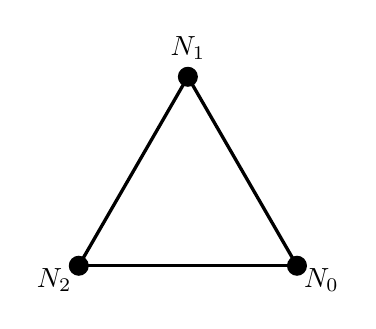
\begin{tikzpicture}[scale=0.8]
                    \foreach \n in {0,...,2}{
                        \draw[very thick] ({-120*\n-30}:2)--({-120*(\n+1)-30}:2) node[midway,sloped,allow upside down]{$\blacktriangleright\blacktriangleright\blacktriangleright$};
                        \draw[fill=black] ({-120*\n-30}:2) circle[radius=0.15];
                    }
                    \draw (-30:2.45) node{$N_0$};
                    \draw (90:2.45) node{$N_1$};
                    \draw (210:2.45) node{$N_2$};
                \end{tikzpicture}
                \caption{Quiver of the $\C^3/\Z_3$ daughter theory.}
                \label{fig:Z3quiver}
            \end{figure}
            The adjacency matrix of this quiver is
            \begin{equation}
                A=
                \begin{bmatrix}
                    0 & 3 & 0 \\
                    0 & 0 & 3 \\
                    3 & 0 & 0
                \end{bmatrix}
            \end{equation}
            which is coherent with the fact that the coefficients of the McKay decomposition of $\rho_1\oplus\rho_1\oplus\rho_1$ are
            \begin{align}
                \begin{split}
                    n_{00} &= 0,\quad n_{01} = 3\qquad n_{02}=0,\\
                    n_{10} &= 0,\quad n_{11} = 0,\qquad n_{12}=3,\\
                    n_{20} &= 3,\quad n_{21} = 0,\qquad n_{22}=0.
                \end{split}
            \end{align}

        \subsubsection{Gauge anomaly cancellation}
        
            Finally, let us discuss the gauge anomaly cancellation. Our fields transform under the adjoint representation of $\SU(n)$, under the fundamentals of $\SU(N_i)$ and under the anti-fundamentals of $\SU(N_i)$. The adjoint representation being reel, it is self-conjugate and therefore do not contribute to the anomaly. Fundamentals of $\SU(N_i)$ have a $+1$ contribution to the anomaly and anti-fundamentals of $\SU(N_i)$ have a $-1$ contribution to the anomaly. Anomaly cancellation therefore imposes that the contribution of the fundamental and of the anti-fundamental of $\SU(N_i)$ cancel each other for each $i=0,1,2$, see appendix \eqref{sec:anomalies}. The bi-fundamental representation $(\boldsymbol{\textbf{N}_i},\boldsymbol{\bar{\textbf{N}}_j})$ counts as $N_j$ fundamentals of $\SU(N_i)$ and as $N_i$ anti-fundamentals $\SU(N_j)$. We get the three following conditions:
            \begin{align}
                \SU(N_0) &: N_2-N_1 = 0,\\
                \SU(N_1) &: N_0-N_2 = 0,\\
                \SU(N_2) &: N_1-N_0 = 0.
            \end{align}
            which immediately imply
            \begin{equation}
                N_0=N_1=N_2.
            \end{equation}
            From \eqref{eq:sumNiZ3}, we get that $N_0=N_1=N_2=N/3$, meaning that that the daughter theory has quantum gauge symmetry if and only if the parent theory with has gauge group $\SU(N)$ where $N$ is a multiple of $3$. Or, in other words, if the number of D-branes is a multiple of $3$.

\section{$\mN=2$ daughter theories}

    %Let us consider that $\Gamma$ is a finite subgroup of $\SU(2)\subset\SU(3)$. It naturally acts on $\C^3$ trough its fundamental representation $\bs{2}$ as $\bs{1}\oplus\bs{2}$ (only acts on 2 coordinates).

    \subsection{$S=\C\times\C^2/\Z_n$}

        We consider a representation $(\rho,\C^N)$ of $\Z_n$. We decompose it on the set of irreducible representations of $\Z_n$ as
        \begin{equation}
            (\rho,V)=\bigoplus^{n-1}_{i=0}N_i(\rho_i,V_i).
        \end{equation}
        In other words, it is equivalent to the representation
        \begin{equation}
            \rho(g)=
            \begin{bmatrix}
                1 & & & \cdots & & & 0 \\
                & \ddots & & & & & \\
                & & 1 & & & &  \\
                \vdots & & & \ddots & & & \vdots \\
                & & & & \zeta^{n-1}_n & & \\
                & & & & & \ddots & \\
                0 & & & \cdots & & & \zeta^{n-1}_n 
            \end{bmatrix}
            \hspace{-0.2cm}
            \begin{tabular}{l}
            $\left.\lefteqn{\phantom{
                \begin{matrix}
                    a_0\\ \ddots\\ a_0\ 
                \end{matrix} 
            }}\right\}N_0$\\
            \vdots \\
            $\left.\lefteqn{\phantom{
                \begin{matrix}
                    b_0\\ \ddots\\ b_0\ 
                \end{matrix}
            }} \right\}N_{n-1}$
            \end{tabular}.\label{eq:reprrhoZn}
        \end{equation}
        Since $\dim\rho_i=1$, $\sum_i N_i=N$. 

        The gauge field configurations that are left invariant under the action of $\Z_n$ are therefore the ones that satisfy
        \begin{equation}
            \rho(g)A_\mu\rho(g)^{-1}=A_\mu.
        \end{equation}
        The constrained is easily solved by using the bi-index notation:
        \begin{equation}
            A_{\mu;i\alpha_i,i\beta_j}\mapsto \rho_i(g)A_{\mu;i\alpha_i,j\beta_j}\rho_j(g)^{-1}=\zeta^{i-j}_nA_{\mu;i\alpha_i,j\beta_j}.
        \end{equation}
        thus only the configurations with $A_{\mu;i\alpha_i,j\beta_j}=0$ if $i\neq j$ are invariant. The gauge field has therefore a block diagonal form:
        \begin{equation}
            A_\mu=
            \begin{bmatrix}
                A_{\mu;00} & & & \\
                & A_{\mu;11} & & \\
                & & \ddots & \\
                & & & A_{\mu;n-1,n-1}
            \end{bmatrix}
        \end{equation}
        with $A_{\mu;ij}\equiv (A_{\mu;i\alpha_i,j\beta_j})_{\alpha_i=0,\dots,N_i,\beta_j=0,\dots,N_j}$. The block $A_{ii}$ transforms under $\Z_n$ as $(\rho_i,V_i)^{N_i}$. For now it is only a simple generalization of the case $\C^3/\Z_3$, the first steps are extremely similar. This makes sense: since the gauge field does not transform under R-symmetry, the specific way by which $\Z_n$ acts on $\C^3$ does not matter.
        
        The gauge group is now broken to
        \begin{equation}
            G_{\text{proj}}=\prod^{n-1}_{i=0}~\U(N_i).
        \end{equation}

        Now for the scalar fields. The action of $\Z_n$ that we consider leaves the first component of $\C^3$ untouched so we take the action $\boldsymbol{1}\oplus\boldsymbol{2}$ where $\boldsymbol{2}$ is the usual action of $\Z_n$ on $\C^2$. In other words, 
        \begin{equation}
            R(g)=
            \begin{bmatrix}
                1 & 0 & 0 \\
                0 & \zeta_n & 0 \\
                0 & 0 & \zeta^{-1}_n
            \end{bmatrix}.
        \end{equation}
        Or, equivalently, $R(g)\indices{^m_n}=\delta\indices{^m_n}A_n$ with $A_m=(1,1,\zeta_n,\zeta_n,\zeta^{-1}_n,\zeta^{-1}_n)$. The scalar field configurations that are left invariant satisfy
        \begin{equation}
            R(g)\indices{^m_n}\rho(g)X^n\rho(g)^{-1}=X^m
        \end{equation}
        for all $g\in\Z_n$. Using the bi-index notations, this becomes
        \begin{align}
            X^m_{i\alpha_i,j\beta_j}\mapsto  \delta\indices{^m_n}A_n\rho_i(g)X^m_{i\alpha_i,j\beta_j}\rho_j(g)^{-1}  = \delta\indices{^m_n}A_n\zeta^{i-j}_n X^m_{i\alpha_i,j\beta_j} =
            \begin{cases}
                \zeta^{i-j}_nX^m_{i\alpha_i,j\beta_j},\quad m=0,1\\
                \zeta^{i-j+1}_nX^m_{i\alpha_i,j\beta_j},\quad m=2,3\\
                \zeta^{i-j-1}_nX^m_{i\alpha_i,j\beta_j},\quad m=4,5\\
            \end{cases}\\
            \bar{X}^m_{i\alpha_i,j\beta_j}\mapsto \delta\indices{^m_n}\bar{A_n}\rho_i(g)\bar{X}^m_{i\alpha_i,j\beta_j}\rho_j(g)^{-1}  = \delta\indices{^m_n}\bar{A_n}\zeta^{i-j}_n X^m_{i\alpha_i,j\beta_j} =
            \begin{cases}
                \zeta^{i-j}_nX^m_{i\alpha_i,j\beta_j},\quad m=0,1\\
                \zeta^{i-j-1}_nX^m_{i\alpha_i,j\beta_j},\quad m=2,3\\
                \zeta^{i-j+1}_nX^m_{i\alpha_i,j\beta_j},\quad m=4,5\\
            \end{cases}
        \end{align}
        thus only the configurations with $X^{0,1}_{i\alpha_i,j\beta_j}=0$ if $i-j\neq0$, $X^{2,3}_{i\alpha_i,j\beta_j}=0$ if $i-j+1\neq0$ and $X^{4,5}_{i\alpha_i,j\beta_j}=0$ if $i-j-1\neq0$ are left invariant (and similarly for the conjugated fields). The scalar fields $X$ have a the following forms:
        {\small
        \begin{align}
            X^{0,1}&=
            \begin{bmatrix}
                X^{0,1}_{00} &  & 0 \\
                 & \ddots & \\
                0 & & X^{0,1}_{n-1,n-1}
            \end{bmatrix},\\
            X^{2,3}&=
            \begin{bmatrix}
                0 & X^{2,3}_{01} & & 0 \\
                 & \ddots & \ddots & \\
                 & & 0 & X^{2,3}_{n-2,n-1} \\
                X^{2,3}_{n-1,0} & & & 0 
            \end{bmatrix},\quad
            X^{4,5}=
            \begin{bmatrix}
                0 & & & X^{4,5}_{0,n-1} \\
                X^{4,5}_{10} & 0 & & \\
                 & \ddots & \ddots  & \\
                0 & & X^{4,5}_{n-1,n-2} & 0
            \end{bmatrix},\\
            \bar{X}^{0,1}&=
            \begin{bmatrix}
                \bar{X}^{0,1}_{00} &  & 0 \\
                 & \ddots & \\
                0 & & \bar{X}^{0,1}_{n-1,n-1}
            \end{bmatrix},\\
            \bar{X}^{2,3}&=
            \begin{bmatrix}
                0 & & & \bar{X}^{2,3}_{0,n-1} \\
                \bar{X}^{2,3}_{10} & 0 & & \\
                 & \ddots & \ddots  & \\
                0 & & \bar{X}^{2,3}_{n-1,n-2} & 0
            \end{bmatrix},\quad
            \bar{X}^{4,5}=
            \begin{bmatrix}
                0 & \bar{X}^{4,5}_{01} & & 0 \\
                 & \ddots & \ddots & \\
                 & & 0 & \bar{X}^{4,5}_{n-2,n-1} \\
                 \bar{X}^{4,5}_{n-1,0} & & & 0
            \end{bmatrix}
        \end{align}}
        so $X^m_{ij}$ is an $N_i\times N_j$ block and transforms under the representation $(\boldsymbol{\textbf{N}_i},\boldsymbol{\bar{\textbf{N}}_j})$ of $\U(N_i)\times\U(N_j)$:
        \begin{align}
            X^{0,1}_{i,i} &\in \boldsymbol{\textbf{N}_i}\otimes\boldsymbol{\bar{\textbf{N}}_i} \cong \Hom(V_i,V_i),\\
            X^{2,3}_{i,i+1} &\in \boldsymbol{\textbf{N}_{i+1}}\otimes\boldsymbol{\bar{\textbf{N}}_i} \cong \Hom(V_{i+1},V_i),\\
            X^{4,5}_{i+1,i} &\in \boldsymbol{\textbf{N}_i}\otimes\boldsymbol{\bar{\textbf{N}}_{i+1}} \cong \Hom(V_i,V_{i+1}).
        \end{align}
        So the scalar fields are split up in three families depending on the way they transform under a gauge transformation. We now see a big difference with the case $\C^3/\Z_3$: since the R-symmetry does not act the same way on each directions in $\C^3$, the invariant scalar field configurations are not the same in each direction either.

        Let us draw the quiver for the case $n=3$ so that we can compare to \ref{fig:Z3quiver}. We have $2\cdot 9=18$ real scalar fields in $9$ different representations:
        \begin{align}
            X^0_{00},X^1_{00}&\in(\boldsymbol{\textbf{N}_0},\boldsymbol{\bar{\textbf{N}}_0}),\quad
            X^0_{11},X^1_{11}\in(\boldsymbol{\textbf{N}_1},\boldsymbol{\bar{\textbf{N}}_1}),\quad
            X^0_{22},X^1_{22}\in(\boldsymbol{\textbf{N}_2},\boldsymbol{\bar{\textbf{N}}_2}),\\
            X^2_{01},X^3_{01}&\in(\boldsymbol{\textbf{N}_1},\boldsymbol{\bar{\textbf{N}}_0}),\quad
            X^2_{12},X^3_{12}\in(\boldsymbol{\textbf{N}_2},\boldsymbol{\bar{\textbf{N}}_1}),\quad
            X^2_{20},X^3_{20}\in(\boldsymbol{\textbf{N}_0},\boldsymbol{\bar{\textbf{N}}_2}),\\
            X^4_{10},X^5_{10}&\in(\boldsymbol{\textbf{N}_0},\boldsymbol{\bar{\textbf{N}}_1}),\quad
            X^4_{21},X^5_{21}\in(\boldsymbol{\textbf{N}_1},\boldsymbol{\bar{\textbf{N}}_2}),\quad
            X^4_{02},X^5_{02}\in(\boldsymbol{\textbf{N}_2},\boldsymbol{\bar{\textbf{N}}_0}),
        \end{align}
        We now only have 1 complex scalar in each representation and the quiver is given by \ref{fig:2Z3quiver}.
        \begin{figure}[H]
            \centering
            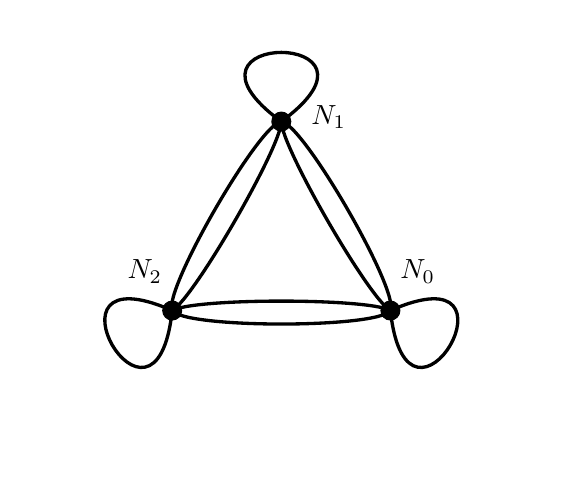
\begin{tikzpicture}[scale=0.8]
                \foreach \n in {0,...,2}{
                    \draw[very thick] ({120*\n-30}:2) .. controls ({120*\n-20}:2) and ({120*\n+120-40}:2) .. ({120*\n+120-30}:2) node[midway,sloped,allow upside down]{$\blacktriangleright$};
                    \draw[very thick] ({120*\n-30}:2) .. controls ({120*\n-30}:1.6) and ({120*\n+120-30}:1.6) .. ({120*\n+120-30}:2) node[midway,sloped,allow upside down]{$\blacktriangleleft$};
                    \draw[very thick] ({120*\n-30}:2) .. controls ({120*\n}:4) and ({120*\n-60}:4) .. ({120*\n-30}:2) node[midway,sloped,allow upside down]{$\blacktriangleright$};
                    \draw[fill=black] ({120*\n-30}:2) circle[radius=0.15];
                }
                \draw (-10:2.2) node{$N_0$};
                \draw (70:2.2) node{$N_1$};
                \draw (190:2.2) node{$N_2$};
            \end{tikzpicture}
            \caption{Quiver of the $\C\times\C^2/\Z_3$ daughter theory.}
            \label{fig:2Z3quiver}
        \end{figure}
        It is easy to see how the construction of the the quiver generalizes for arbitrary $n$. The adjacency matrix is
        \begin{equation}
            A=
            \begin{bmatrix}
                1 & \cdots & 1 \\
                \vdots & \ddots & \vdots \\
                1 & \cdots & 1
            \end{bmatrix}
        \end{equation}
        which is, as it should, coincides with the McKay decomposition of $\boldsymbol{1}\oplus\boldsymbol{2}$:
        \begin{align}
            \begin{split}
                n_{00} &= 1,\quad\dots,\qquad n_{0,n-1}=1,\\
                &\vdots\hspace{3.7cm}\vdots\\
                n_{n-1,0} &= 1,\quad\dots,\qquad n_{n-1,n-1}=1.
            \end{split}
        \end{align}
        
        Gauge anomaly cancellation now imposes that
        \begin{equation}
            N_{i-1}-N_{i-1}+N_{i+1}+N_{i+1}=0
        \end{equation}
        for $i=0,\dots,n-1$. Those constrains are always satisfied so the the factors $N_i$ are arbitrary, as long as $\sum_iN_i=N$ of course.

    \subsection{$S=\C\times\C^2/\D_n$}

        We quotient $\C^3$ by the binary dihedral group $\D_n$ that acts on the last two components. A set of irreducible representations of $\D_n$ is given by
        \begin{equation}
            \{(\rho_i,V_i)\}_{i=0,\dots,n+2}
        \end{equation}
        with $V_i=\C$ for $i=0,\dots,3$ and $V_i=\C^2$ for $i=4,\dots,n+2$, so there are $4$ one-dimensional representations and $n-1$ two-dimensional representations. They are explicitely given in section \ref{sec:irrep}. Using the bi-index notations $A_{\mu;i\alpha_i,j\beta_j}$ with $i,j=0,\dots,n+2$ and $\alpha_i,\beta_j=0,\dots,\dim\rho_i\cdot N_i-1$, the invariant configurations must have $A_{\mu;ij}=0$ if $i\neq j$, i.e. it must have a diagonal block-form, wiht block of size $\N_i\times N_i$ for $i=0,\dots,3$ and of size $2N_i\times 2N_i$ for $i=4,\dots,n+1$. The blocks transforming under the $2$-dimensional representations must have the form
        \begin{equation}
            A_{\mu;ii}=
            \begin{bmatrix}
                A_{\mu;i0,i0} & A_{\mu;i0,i1} & \cdots & A_{\mu;i,0,i,2N_i-2} & A_{\mu;i,0,i,2N_i-1} \\ 
                \mp A_{\mu;i0,i1} & A_{\mu;i0,i0} & \cdots & \mp A_{\mu;i,0,i,2N_i-1} & A_{\mu;i,0,i,2N_i-2} \\
                \vdots & \cdots & \ddots & \vdots & \vdots \\
                A_{\mu;i,2N_i-2,i,0} & A_{\mu;i,2N_i-2,i1} & \cdots & A_{\mu;i,2N_i-2,i,2N_i-2} & A_{\mu;i,2N_i-2,i,2N_i-1} \\ 
                \mp A_{\mu;i,2N_i-2,i1} & A_{\mu;i,N_i-2,i,0} & \cdots & \mp  A_{\mu;i,2N_i-2,i,2N_i-1} & A_{\mu;i,2N_i-2,i,2N_i-2}
            \end{bmatrix}
        \end{equation}
        so each block is composed of $N^2_i$ $2\times2$ matrices of the form
        \begin{equation}
            \begin{bmatrix}
                A & B \\
                \mp B & A
            \end{bmatrix}.
        \end{equation}
        We take the ``$-$'' signs when $i$ is even and the ``$+$'' signs when $i$ is odd. This comes from the fact that the $2$-dimensional representations involve alternating signs.

        R-symmetry acts on the three complex scalar fields as
        \begin{equation}
            R(A) =
            \begin{matrix}
                A
            \end{matrix}
        \end{equation}

    \subsection{$S=\C\times\C^2/\T$}

    \subsection{$S=\C\times\C^2/\mathcal{O}$}

    \subsection{$S=\C\times\C^2/\I$}






\section{$\mN=1$ daughter theories}

    \subsection{$S=\C^3/\Z_n$}

        Let us now consider the general case of $\Z_n$ acting on $\C^3$, i.e. we want to generalize the case that we treated in section \ref{sec:C3Z3}. 
        
        \subsubsection{Actions of $\Z_n$ on $\C^3$}
        
            The first thing to do is to specify a representation of $\Z_n$ on $\C^3$. Any representation $(R,\C^3)$ can be decomposed as
            \begin{equation}
                R=\bigoplus^{n-1}_{k=0} \rho^{\oplus n_k}_k
            \end{equation}
            and is therefore equivalent to a block-diagonal representation. So $R$ can be taken to be
            \begin{equation}
                R(g)=
                \begin{bmatrix}
                    \zeta^a_n & 0 & 0 \\
                    0 & \zeta^b_n & 0 \\
                    0 & 0 & \zeta^c_n
                \end{bmatrix}\label{eq:reprZnC3}
            \end{equation}
            and unitary, with $a,b,c$ some arbitrary exponents. We denote the representation \eqref{eq:reprZnC3} by $(a,b,c)$.  Unitarity imposes that
            \begin{equation}
                (a+b+c)\mod n = 0.\label{eq:cdtabc}
            \end{equation}
            Note that swapping $a,b$ and $c$ will give equivalent representations so we can restrict ourselves to $a\leq b\leq c$. Furthermore, taking $a$ or $a+n$ gives the same representation and the same is true for $b$ and $c$, so we we can actually restrict ourselves to $0<a\leq b\leq c<n$. We can trade the strict inequalities and allow the values $0$ or $n$ if we want to consider trivial representations as well. In this case, we will find that at least one direction of $\C^3$ is left untouched, i.e. we are in the situation where the orbifold is actually $\C\times\C^2/\Z_n$, which we will not consider here.

            The problem has now been reformulated as follows:
            we are looking for all possible ordered triplets $(a,b,c)$ such that $0<a\leq b\leq c<n$ and \eqref{eq:cdtabc}. For $n=1$ and $n=2$, it is clear that this is not possible, the possibilities involve at least one trivial representation. For $n=3$, the only possibility is $(1,1,1)$, the one we used in \ref{sec:C3Z3}. What about bigger values of $n$? First, note that because of \eqref{eq:cdtabc}, the only two possibilities are that $a+b+c$ is equal to $n$ or $2n$. Since we can ignore the case were it is equal to $2n$ (redundant\marker), we find that the maximum value that $a$ can take is $\lfloor n/3\rfloor$, so $a=1,\dots,\lfloor n/3\rfloor$. $c$ can then be expressed in terms of $a$ and $b$ as $c=n-a-b$. The constraint $b\leq c$ then implies $b\leq (n-a)/2$, i.e. $b=a,\dots,\lfloor (n-a)/2\rfloor$. To summarize, the representations are all the representations of the form $(a,b,n-a-b)$ with $a=1,\dots,\lfloor n/3\rfloor$ and $b=a,\dots,\lfloor (n-a)/2\rfloor$. For small values, we get
            \begin{align*}
                \Z_1 &: \text{necessarily involves a trivial representation}\\
                \Z_2 &: \text{necessarily involves a trivial representation}\\
                \Z_3 &: (1,1,1)\\
                \Z_4 &: (1,1,2)\\
                \Z_5 &: (1,1,3),(1,2,2)\label{reprZ5C3}\\
                \Z_6 &: (1,1,4),(1,2,3),(2,2,2)\\
                \Z_7 &: (1,1,5),(1,2,4),(1,3,3),(2,2,3)\\
                &\vdots
            \end{align*}
            For an arbitrary $n$, the total number of different representation is
            \begin{equation}
                \sum^{\lfloor n/3\rfloor}_{a=1}~\left\lfloor \frac{n-3a}{2}+1\right\rfloor = \begin{cases}
                    3k^2,\qquad\text{if $n=6k$}\\
                    3k^2+k,\qquad\text{if $n=6k+1$},\\
                    3k^2+2k,\qquad\text{if $n=6k+2$},\\
                    3k^2+3k+1,\qquad\text{if $n=6k+3$},\\
                    3k^2+4k+1,\qquad\text{if $n=6k+4$},\\
                    3k^2+5k+2,\qquad\text{if $n=6k+5$}
                \end{cases}
            \end{equation}
            The details are presented in appendix \ref{app:compsum}.

        \subsubsection{Example: $\Z_5$}

            For $\Z_5$, we saw that there are two nonequivalent ways of acting on $\C^3$, see \eqref{reprZ5C3}. Let us first consider the action $(1,1,3)$
            \begin{equation}
                R(g)=
                \begin{bmatrix}
                    \zeta_5 & 0 & 0\\
                    0 & \zeta_5 & 0\\
                    0 & 0 & \zeta^3_5
                \end{bmatrix}
            \end{equation}
            i.e. $R=\rho_1\oplus\rho_1\oplus\rho_3$.

            For the gauge field, the reasoning is exactly the same than for $\Z_3$ and we get
            \begin{equation}
                A_\mu=
                \begin{bmatrix}
                    A_{\mu;00} & & \\
                    & \ddots & \\
                    & & A_{\mu;44}
                \end{bmatrix}
            \end{equation}
            where each block $A_{\mu;ii}$ is of size $N_i\times N_i$. The projected gauge group is
            \begin{equation}
                G_{\text{proj}} = \U(N_0)\times\U(N_1)\times\U(N_2)\times\U(N_3)\times\U(N_4).
            \end{equation}

            The scalar fields transform as
            \begin{equation}
                X^m_{i\alpha_i,j\beta_j}\to R(g)\indices{^m_n}\rho_i(g)X^n_{i\alpha_i,j\beta_j}\rho_j(g)^{-1}
            \end{equation}
            so the invariant configurations must satisfy
            \begin{equation}
                X^m_{i\alpha_i,j\beta_j} = R(g)\indices{^m_n}\zeta^{i-j}_4\rho_i(g)X^n_{i\alpha_i,j\beta_j} = 
                \begin{cases}
                    \zeta^{i-j+1}X^m_{i\alpha_i,j\beta_j},\quad\text{if } m=0,1,2,3\\
                    \zeta^{i-j+3}X^m_{i\alpha_i,j\beta_j},\quad\text{if } m=4,5.
                \end{cases}
            \end{equation}
            and are therefore of the form
            \begin{equation}
                X^m = 
                \begin{bmatrix}
                    0 & X^m_{01} & 0 & 0 & 0\\
                    0 & 0 & X^m_{12} & 0 & 0\\
                    0 & 0 & 0 & X^m_{23} & 0\\
                    0 & 0 & 0 & 0 & X^m_{34}\\
                    X^m_{40} & 0 & 0 & 0 & 0
                \end{bmatrix}
            \end{equation}
            for $m=0,1,2,3$ and 
            \begin{equation}
                X^m = 
                \begin{bmatrix}
                    0 & 0 & 0 & X^m_{03} & 0\\
                    0 & 0 & 0 & 0 & X^m_{14}\\
                    X^m_{20} & 0 & 0 & 0 & 0\\
                    0 & X^m_{31} & 0 & 0 & 0\\
                    0 & 0 & X^m_{42} & 0 & 0
                \end{bmatrix}
            \end{equation}
            for $m=4,5$. Gauge anomaly cancellation imposes
            \begin{align}
                -N_{i-2}+N_{i+2}-2N_{i+1}+2N_{i-1}=0
            \end{align}
            for $i=0,1,2,3,4$ which implies that
            \begin{equation}
                N_0=N_1=N_2=N_3=N_4.
            \end{equation}

            Now if we choose the representation $(1,2,2)$, i.e.
            \begin{equation}
                R(g)=
                \begin{bmatrix}
                    \zeta_5 & 0 & 0\\
                    0 & \zeta^2_5 & 0\\
                    0 & 0 & \zeta^2_5
                \end{bmatrix}
            \end{equation}
            we get instead that the invariant field configurations must satisfy
            \begin{equation}
                X^m_{i\alpha_i,j\beta_j} = R(g)\indices{^m_n}\zeta^{i-j}_4\rho_i(g)X^n_{i\alpha_i,j\beta_j} =
                \begin{cases}
                    \zeta^{i-j+1}X^m_{i\alpha_i,j\beta_j},\quad\text{if } m=0,1\\
                    \zeta^{i-j+2}X^m_{i\alpha_i,j\beta_j},\quad\text{if } m=2,3,4,5.
                \end{cases}
            \end{equation}
            and are therefore of the form
            \begin{equation}
                X^m = 
                \begin{bmatrix}
                    0 & X^m_{01} & 0 & 0 & 0\\
                    0 & 0 & X^m_{12} & 0 & 0\\
                    0 & 0 & 0 & X^m_{23} & 0\\
                    0 & 0 & 0 & 0 & X^m_{34}\\
                    X^m_{40} & 0 & 0 & 0 & 0
                \end{bmatrix}
            \end{equation}
            for $m=0,1$ and 
            \begin{equation}
                X^m = 
                \begin{bmatrix}
                    0 & 0 &  X^m_{02} & 0 & 0\\
                    0 & 0 & 0 &  X^m_{13} & 0\\
                    0 & 0 & 0 & 0 &  X^m_{24}\\
                    X^m_{30} & 0 & 0 & 0 & 0\\
                    0 &  X^m_{41} & 0 & 0 & 0
                \end{bmatrix}
            \end{equation}
            for $m=2,3,4,5$. Gauge anomaly cancellation imposes
            \begin{align}
                -2N_{i+2}+2N_{i-2}-N_{i+1}+N_{i-1}=0\marker
            \end{align}
            for $i=0,1,2,3,4$ which implies that
            \begin{equation}
                N_0=N_1=N_2=N_3=N_4.
            \end{equation}

            \begin{figure}
                \centering
                \begin{subfigure}[b]{0.3\textwidth}
                    \centering
                    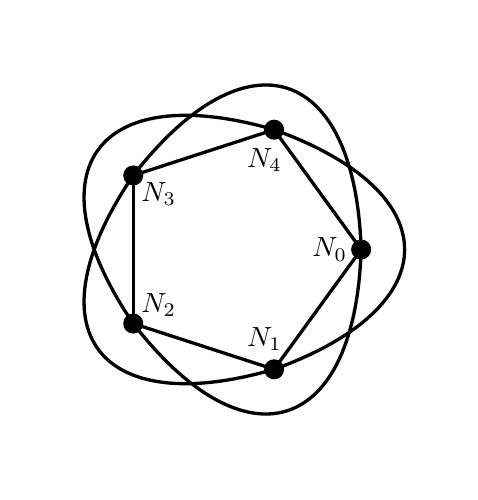
\begin{tikzpicture}[scale=0.8]
                        \foreach \n in {0,...,4}{
                            \draw[very thick] (-72*\n:2) .. controls ({-72*(\n+1)+15}:3.5) and ({-72*(\n+1)-15}:3.5) .. ({-72*(\n+2)}:2) node[midway,sloped,allow upside down]{$\blacktriangleright$};
                            \draw[very thick] ({-72*\n}:2) -- ({-72*(\n-1)}:2) node[midway,sloped,allow upside down]{$\blacktriangleright\blacktriangleright$};
                            \draw[fill=black] (-72*\n:2) circle[radius=0.15];
                            \draw (-72*\n:1.5) node{$N_\n$};
                        }
                    \end{tikzpicture}
                    \caption{$(1,1,3)$}
                    \label{fig:y equals x}
                \end{subfigure}
                \hspace{2cm}
                \begin{subfigure}[b]{0.3\textwidth}
                    \centering
                    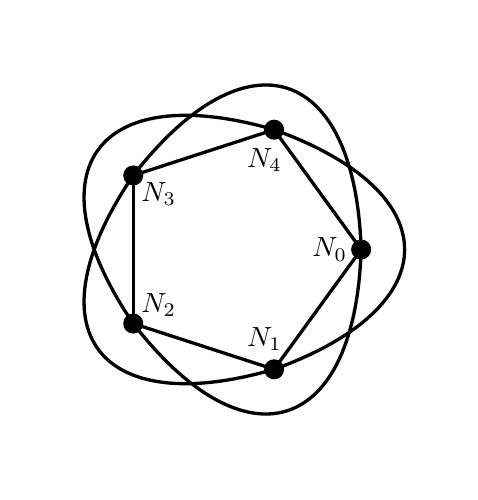
\begin{tikzpicture}[scale=0.8]
                        \foreach \n in {0,...,4}{
                            \draw[very thick] (-72*\n:2) .. controls ({-72*(\n+1)+15}:3.5) and ({-72*(\n+1)-15}:3.5) .. ({-72*(\n+2)}:2) node[midway,sloped,allow upside down]{$\blacktriangleleft\blacktriangleleft$};
                            \draw[very thick] ({-72*\n}:2) -- ({-72*(\n-1)}:2) node[midway,sloped,allow upside down]{$\blacktriangleright$};
                            \draw[fill=black] (-72*\n:2) circle[radius=0.15];
                            \draw (-72*\n:1.5) node{$N_\n$};
                        }
                    \end{tikzpicture}
                    \caption{$(1,2,2)$}
                    \label{fig:three sin x}
                \end{subfigure}
                \caption{Quivers of the $\C^3/\Z_5$ daughter theories.}
                \label{fig:three graphs}
           \end{figure}



        

    \subsection{$S=\C^3/(\Z_m\times\Z_n)$}




    \section{Summary of daughter theories}

    \begin{table}[H]
        \centering
        {\small
        $
        \begin{array}{|c|c|c|l|c|c|}
            \hline
            S & \mN & \text{Gauge group} & \text{Field content} & \text{Quiver} & \begin{tabular}{@{}l@{}} \text{Gauge anomaly} \\ \text{constraint}  \end{tabular} \\ \hline
            \C^3 & 4 & \U(N) & \begin{tabular}{@{}l@{}}$A_\mu\in\Hom(\C^n,\C^n)$  \\ $\phi\in\boldsymbol{6}\otimes\Hom(\C^n,\C^n)$ \\ $\psi\in\boldsymbol{4}\otimes\Hom(\C^n,\C^n)$ \end{tabular} & &  \\ \hline
            \C\times\C^2/\Z_3 & 2 & & & \begin{tikzpicture}[baseline={($ (current bounding box.center) - (0,3pt) $)},scale=0.4]
                \foreach \n in {0,...,2}{
                    \draw[very thick] ({120*\n-30}:2) .. controls ({120*\n-20}:2) and ({120*\n+120-40}:2) .. ({120*\n+120-30}:2) node[midway,sloped,allow upside down]{\tiny{$\blacktriangleright$}};
                    \draw[very thick] ({120*\n-30}:2) .. controls ({120*\n-30}:1.6) and ({120*\n+120-30}:1.6) .. ({120*\n+120-30}:2) node[midway,sloped,allow upside down]{\tiny{$\blacktriangleleft$}};
                    \draw[very thick] ({120*\n-30}:2) .. controls ({120*\n}:4) and ({120*\n-60}:4) .. ({120*\n-30}:2) node[midway,sloped,allow upside down]{\tiny{$\blacktriangleright$}};
                    \draw[fill=black] ({120*\n-30}:2) circle[radius=0.15];
                }
                \draw (0:2.2) node{$N_0$};
                \draw (60:2.2) node{$N_1$};
                \draw (180:2.2) node{$N_2$};
            \end{tikzpicture} & \\ \hline
            \C\times\C^2/\D_n & 2 & & & & \\ \hline
            \C\times\C^2/\T & 2 & & & & \\ \hline
            \C\times\C^2/\O & 2 & & & & \\ \hline
            \C\times\C^2/\I & 2 & & & & \\ \hline
            \C^3/\Z_3 & 1 & \U(N_0)\times\U(N_1)\times\U(N_2) & \begin{tabular}{@{}l@{}}$A_\mu\in\marker$ \\ $X^m_{01}\in\Hom(V_1,V_0)$ \\ $X^m_{12}\in\Hom(V_2,V_1)$ \\$ X^m_{20}\in\Hom(V_0,V_2)$ \\ $\psi\in\marker$\end{tabular} &
            \begin{tikzpicture}[baseline={($ (current bounding box.center) - (0,3pt) $)},scale=0.4]
                \foreach \n in {0,...,2}{
                    \draw[very thick] ({-120*\n-30}:2)--({-120*(\n+1)-30}:2);
                    \draw[fill=black] ({-120*\n-30}:2) circle[radius=0.15];
                    \draw ({120*\n+30}:1) node[rotate={120*\n-60}]{\tiny{$ \blacktriangleright\blacktriangleright\blacktriangleright$}};
                }
                \draw (-30:2.7) node{$N_0$};
                \draw (90:2.7) node{$N_1$};
                \draw (210:2.7) node{$N_2$};
            \end{tikzpicture} & N_0=N_1=N_2 \\ \hline
        \end{array}
        $}
        \caption{List of worldvolume theories for different transverse spaces.}
    \end{table}


\section{Generalizations}

    Let us discuss the different ways our previous discussions can be generalized.

    \subsection{$(p+1)$-dimensional quiver gauge theories}

        First, we can generalize our initial brane-world paradigm and consider D$p$-branes in type II string theory (type IIA if $p$ is even and type IIB if $p$ is odd) instead of just D$3$-branes. The spacetime is then of the form
        \begin{equation}
            M = \R^{1,p}\times\R^{9-p}/\Gamma
        \end{equation}
        where $\Gamma$ is a discrete subgroup of $\Spin(9-p)$. If $\Gamma$ is a subgroup of a special holonomy group, we recover a somewhat generalized version of the paradigm that we discussed above. In this case the transverse space is a Calabi-Yau orbifold and some degree of supersymmetry is preserved. Note that the fermionic and bosonic quivers that coincides. If $\Gamma$ is not a subgroup os a special holonomy group, then the $(p+1)$-dimensional quiver gauge theory that we obtain in the low-energy limit is not supersymmetric. We then have different quivers for the fermions and the bosons, although with the same vertices, by definition.

        One can also consider replacing the orbifold by a conifold by deforming singular algebraic description of the orbifold with a field into a family smooth surfaces. The total space is then the conifold.

    \subsection{Projective representations and discrete torsion}

    \subsection{Quiver gauge theories deformations and conifold}

\pagebreak
\appendix

\section{Gauge anomaly}\label{sec:anomalies}

    The \emph{anomaly degree} $A(\rho)$ of a representation $\rho$ is defined as
    \begin{equation}
        \frac{1}{2}\tr(T_a\{T_b,T_c\})=A(\rho)d_{abc}
    \end{equation}
    where $d_{abc}$ is an invariant symmetric tensor of the Lie algebra of $G$, independent of the representation. One can show that $A(\rho^*)=-A(\rho)$ so self dual representation have $A(\rho)=0$ in particular. The only simple Lie groups that allow for a complex non-self-conjugate representation are $\SU(n)$ with $n\geq3$. We can normalize $d_{abc}$ such that $A(\rho)=1$ for the fundamental $n$-dimensional representations.

\section{Reminder on $\mN=4$ super Yang-Mills theory in $D=4$}\label{sec:N4SCFT}

    \subsection{Superconformal group $\SU(2,2|4)$ and its representations}

        Conformal transformations and supersymmetries do not commute so the presence of conformal symmetry in addition to $\mN=4$ supersymmetry leads to an even larger group of symmetry known as the \emph{superconformal group}. In the $D=4,\mN=4$ case, the superconformal group is the super group\footnote{Supermanifold which is also a group with smooth product and inverse maps.} $\SU(2,2|4)$. The different component of the latter are
        \begin{itemize}
            \item \textbf{Conformal symmetries}: they form the 15-dimensional subgroup $\SO(2,4)$ and are generated by $P_\mu,M_{\mu\nu},K_\mu$ and $D$.
            \item \textbf{R-symmetry}: they form the 15-dimensional subgroup $\SO(6)_R$ and are generated by $T^A$ ($A=1,\dots,15$).
            \item \textbf{Poincaré supersymmetries}: they form the 16-dimensional sub group \marker and are generated by $Q^I_\alpha$ and $\bar{Q}^I_{\dalpha}$.
            \item \textbf{Conformal supersymmetries}: they form the 16-dimensional subgroup \marker and are generated by $S_{\alpha I}$ and $\bar{S}^{\dalpha I}$.
        \end{itemize}

        Conformal invariance of this theory can be seen as a consequence of the non-renormalization theorems.

    \subsection{Matter content}
        
        For $D=4,\mN=4$, there is one kind of supermultiplet, the vector multiplet. The decomposition of the $\mN = 4$ vector superfield in terms of $\mN = 1$ representations is as follows:
        \begin{equation}
            [\mN = 4 \text{ vector multiplet}] : V = (\lambda_\alpha, A_\mu, D) \oplus \Phi^A = (\phi^A,\psi^A_\alpha,F^A).
        \end{equation}
        with $A=1,2,3$, i.e. in terms of one vector supermultiplet and three chiral scalar supermultiplets. The propagating degrees of freedom are therefore a vector field, six scalars and four gauginos.
        
        The Lagrangian is very much constrained by $\mN = 4$ supersymmetry. First, the chiral superfields $\Phi^A$ should transform in the adjoint representation of the gauge group $G$, since internal symmetries commute with supersymmetry. This means that all fields transform in the adjoint of $G$.
        
        Moreover, there is a large R-symmetry group, $\SU(4)_R$. The four Weyl fermions transform in the fundamental of $\SU(4)_R$, while the six real scalars in the two times anti-symmetric representation, which is nothing but the fundamental representation of $\SO(6)$. The auxiliary fields are singlets under the R-symmetry group. Using $\mN = 1$ superfield formalism the Lagrangian reads
        \begin{align}
            \begin{split}
                \L^{\mN=4}_{\text{SYM}} &= \frac{1}{32\pi}\Im \left(\tau\int\d^4x\tr(W^\alpha W_\alpha)\right)+\int\d^2\theta\d^2\bar{\theta}\tr\sum^3_{A=1}\bar{\Phi}^Ae^{2gV}\Phi^A\\
                &\quad-\int\d^2\theta\sqrt{2g}\tr\Phi_1[\Phi_2,\Phi_3]+\text{h.c.}
            \end{split}\label{eq:N4lag}
        \end{align}
        where the commutator in the third term appears for the same reason as for the $\mN = 2$ Lagrangian. Notice that the choice of a single $\mN = 1$ supersymmetry generator breaks the full $\SU(4)_R$ R-symmetry to $\SU(3)\times \U(1)_R$. The three chiral superfields transform in the $\boldsymbol{3}$ of $\SU(3)$ and have R-charge $R = 2/3$ under the $\U(1)_R$. It is an easy but tedious exercise to perform the integration in superspace and get an explicit expression in terms of fields. Finally, one can solve for the auxiliary fields and get an expression where only propagating degrees of freedom are present, and where $\SU(4)_R$ invariance is manifest (the fact that the scalar fields transform under the fundamental representation of $\SO(6)$, which is real, makes the R-symmetry group of the $\mN = 4$ theory being at most $\SU(4)$ and not $\U(4)$, in fact).

    \subsection{Dynamical phases}

        The scalar potential in \eqref{eq:N4lag} can be written in a rather compact form in terms of the six real scalars $X^i$ making up the three complex scalars $\phi^A$ and reads
        \begin{equation}
            V = \frac{1}{2}g^2\tr\sum^6_{i,j=1}[X_i,X_j]^2.
        \end{equation}
        The positive definite behavior of the Cartan-Killing form on the compact gauge algebra $\g$ implies that each term in the sum is positive or zero. In other words, $V=0$ is equivalent to
        \begin{equation}
            [X^i,X^j]=0,\qquad i,j=1,\dots,6.
        \end{equation}
        This equations admit two classes of solutions:
        \begin{itemize}
            \item $\langle X^i\rangle=0$ for all $i=1,\dots,6$. This is the \emph{superconformal phase}. Neither the gauge symmetry nor the superconformal symmetry is broken. The physical states and operators are gauge invariant and transform under
            unitary representations of $\SU(2,2|4)$.
            \item  $\langle X^i\rangle\neq0$ for at least one $i$. This is the \emph{spontaneously broken Coulomb phase}. The gauge algebra $\g$ is going to be broken to $\U(1)^r$, where $r\equiv\rank\g$. The low energy behavior is then the one of $r$ copies of $\mN=4$ $\U(1)$ gauge theories. Superconformal symmetry is spontaneously broken since the non-zero VEV $\langle X^i\rangle$ sets a scale.
        \end{itemize}

        \begin{result}
            \textbf{$\boldsymbol{\mN=4}$ Yang-Mills theory.} There is only one $D=4,\mN=4$ Yang-Mills theory and it contains $3$ $\mN=1$ chiral scalar supermutliplet and $1$ $\mN=1$ vector supermultiplet (up to $g$ and $\tau$). This theory is conformal and can be recovered from dimensional reduction of $D=10,\mN=1$ Yang-Mills on $\mathbb{T}^6$.
        \end{result}

\section{Calabi-Yau compactification}\label{sec:appCY}

    Requireing $\mN=1$ supersymmetry is equivalent too asking that that the configuration resulting from compactification has at least one Killing spinor (covariantly constant spinor). This constant spinor then defines a residual supersymmetry by contracting with the local supersymmetry current. On real $6$-folds, spinors transform under $\SO(6)$. We are therefore looking for the biggest subgroup of $\SO(6)$ that leaves a component of the spinor invariant. In that case the spinor $(1,0,0,0)$ is covariantly conserved, i.e. is a Killing spinor. Using the fact that $\SO(6)\cong\SU(4)$, can clearly see that this subgroup is $\SU(3)$. Our transverse space must therefore have $\SU(3)$ holonomy such that the parallel transport of the spinor $(1,0,0,0)$ under any closed loop is a lower $\SU(3)$ rotation.

\section{Properties of D-branes in type II theories}

    The minimal irreducible representation in 10 dimensions is a Majorana-Weyl representation of dimension 8. In type II theories, we have $\mN=(1,1)$ for IIA and $\mN=(2,0)$ for IIB. Because of the string origin of the generators, the two supersymmetry generators $\eps_L$ and $\eps_R$ (Majorana-Weyl spinors) satisfy
    \begin{equation}
        \eps_L=\Gamma_{11}\eps_L,\qquad \eps_R=\eta\Gamma_{11}\eps_R
    \end{equation}
    with $\eta=+1$ for IIB and $\eta=-1$ for IIA theory. For a D$p$-brane, the supersymmetry projections is the following:
    \begin{equation}
        \eps_L=\Gamma_0\dots\Gamma_p\eps_R.
    \end{equation}
    In other words, the supersymmetries with generators of the form
    \begin{equation}
        Q_\alpha+\Gamma_0\dots\Gamma_p\bar{Q}_{\dalpha}\label{eq:susypresved}
    \end{equation}
    are preserved by the D$p$-brane while the one with generators of the form
    \begin{equation}
        Q_\alpha-\Gamma_0\dots\Gamma_p\bar{Q}_{\dalpha}\label{eq:susybroken}
    \end{equation}
    are broken. They violate the boundary conditions. Since there is the same number of generators of the form \eqref{eq:susypresved} than of the form \eqref{eq:susybroken}, exactly haf of the supersymmetry is broken. The idea that one spacetime direction would break one supercharge could be reasonable if supersymmetries were transforming as vectors which not the case; supercharges transform as spinors. It would also be incompatible with the T-duality because two branes of different dimensions must have the same number of unbroken supercharges if there is a T-duality relating them: the number of unbroken supercharges is the same for all dual descriptions (a necessary condition for the equivalence). And indeed, in the correct theory, that's the case. Every type II D-brane breaks half of the supercharges.

    To obtain the previous relations, we start by the ones from M-theory and compactify the 11th direction, getting type IIA theory. $\Gamma_{11}$ then plays the role of the chiral projector in 10 dimensions; the supersymmetry parameters are related by $\eps_L=\frac{1}{2}(1+\Gamma_{11})\eps$ and $\eps_R=\frac{1}{2}(1-\Gamma_{11})\eps$. The relations for type IIB theory are then obtained by T-duality. Under a T-duality over the $\hat{i}$ direction, the supersymmetry parameters transform as
    \begin{align*}
        \eps_L &\mapsto \eps_L,\\
        \eps_R &\mapsto \Gamma_i\eps_R.
    \end{align*}
    The tension of a D$p$-brane is given by
    \begin{equation}
        T_{p} = \frac{1}{(2\pi)^pg_sl^{p+1}_s}.
    \end{equation}
    This completely fixes the Newton constant: the tension of electric-magnetic duals must satisfy:
    \begin{equation}
        T_pT_{D-p-4} = \frac{2\pi}{16\pi G_D}.
    \end{equation}
    In ten dimensions, this gives $G_{10}=8\pi^6g^2_sl^8_s$.

    The dualities are defined as follows:
    \begin{align*}
        \text{S-duality} &: g_s\mapsto\frac{1}{g_s},\qquad l^2_s\mapsto g_sl^2_s,\\
        \text{T-duality} &: R\mapsto\frac{l^2_s}{R},\qquad g\mapsto g_s\frac{l_s}{R}.
    \end{align*}

\section{Some finite subgroups}

    \subsection{Finite subgroups of $\SU(2)$ and $\SL(2,\C)$}

        \subsubsection{Finite subgroups}

            The first thing to recall is that every finite subgroup of $\SL(2,\C)$ is isomorphic to a subgroup of $\SU(2,\C)$ and vice-versa, so we equivalently talk about the subgroups of $\SU(2)$. The finite subgroups of $\SU(2)$, called the \emph{binary polyhedral groups}, are the doubles covers of the finite subgroups of $\SO(3)$ that are called \emph{polyhedral groups}. They simply constitutes the symmetries of the Platonic solids. The groups fall into two infinite series, associated to the regular polygons, as well as three exceptional, associated with the 5 regular polyhedra: the tetrahedron (self-dual), the cube (and its dual octahedron), the icosahedron (and its dual dodecahedron).

            More precisely, the finite subgroups of $\SL(2,\C)$ are
            \begin{itemize}
                \item $\Z_n$ : cyclic group of order $n$ ($n\geq2$) generated by
                \begin{equation}
                    \begin{bmatrix}
                        \zeta_m & 0\\
                        0 & \zeta^{-1}_m
                    \end{bmatrix}
                \end{equation}
                \item $2\D_n$ : \emph{binary dihedral groups} (also known as the \emph{dicyclic group}) of order $4n$ ($n\geq1$) generated by
                \begin{equation}
                    A \equiv
                    \begin{bmatrix}
                        \zeta_{2n} & 0\\
                        0 & \zeta^{-1}_{2n}
                    \end{bmatrix}\quad \text{ and }
                    B \equiv 
                    \begin{bmatrix}
                        0 & i\\
                        i & 0
                    \end{bmatrix}
                \end{equation}
                One can show that $A^n=B^2$ and that $AB=BA^{-1}$ so that $2\D_n=\{B^bA^a|0\leq b \leq 3, 0\leq a \leq n-1\}$. This rewriting of the most general element of the group will be useful.
                \item $2\mathcal{T}$ : \emph{binary tetrahedral group} of order $24$ generated by $D_2$ and
                \begin{equation}
                    C \equiv \frac{1}{\sqrt{2}}
                    \begin{bmatrix}
                        \zeta_8 & \zeta^3_8\\
                        \zeta_8 & \zeta^7_8
                    \end{bmatrix}
                \end{equation}
                \item $2\mathcal{O}$ : \emph{binary octahedral group} of order $48$ generated by $\mathcal{T}$ and
                \begin{equation}
                    D \equiv 
                    \begin{bmatrix}
                        \zeta^3_8 & 0\\
                        0 & \zeta^5_8
                    \end{bmatrix}
                \end{equation}
                \item $2\mathcal{I}$ : \emph{binary icosahedral group} of order $120$ generated by
                \begin{equation}
                    E \equiv -\frac{1}{\sqrt{5}}
                    \begin{bmatrix}
                        \zeta^4_5-\zeta_5 & \zeta^2_5-\zeta^3_5\\
                        \zeta^2_5-\zeta^3_5 & \zeta_5-\zeta^4_5
                    \end{bmatrix}\quad \text{ and }
                    F \equiv -\frac{1}{\sqrt{5}}
                    \begin{bmatrix}
                        \zeta^2_5-\zeta^4_4 & \zeta^4_5-1\\
                        1-\zeta_5 & \zeta^3_5-\zeta_5
                    \end{bmatrix}
                \end{equation}
            \end{itemize}
            with $\zeta_m\equiv e^{i\frac{2\pi}{m}}$ such that $(\zeta_m)^m=1$. Note that the orders are all divisible by $2$. This is because the center of $\SU(2)$ is $\Z_2$.

        \subsubsection{Irreducible representations}\label{sec:irrep}

            \begin{itemize}
                \item $\Z_n$ has $n$ irreducible representations. They are all $1$-dimensional (since $\Z_n$ is abelian) and are given by
                \begin{equation}
                    \rho_k(g)=\zeta^k_n
                \end{equation}
                with $k=0,\dots,n-1$.
                \item $2\D_n$ has $n+3$ irreducible representations: $4$ of dimension $1$ and $n-1$ of dimension $2$. The $1$-dimensional ones are given by
                \begin{equation*}
                \begin{array}{|c|c|c|c|}
                    \hline
                    n & \rho(A) & \rho(B) & \rho(B^bA^a) \\
                    \hline
                    \multirow[c]{4}{*}{\text{even}} & \multirow[c]{2}{*}{1} & 1 & 1 \\ \cline{3-4}
                    & & -1 & (-1)^b \\ \cline{2-4}
                    & \multirow[c]{2}{*}{-1} & 1 & (-1)^a \\ \cline{3-4}
                    & & -1 & (-1)^{a+b} \\
                    \hline
                    \multirow[c]{4}{*}{\text{odd}} & \multirow[c]{2}{*}{1} & 1 & 1 \\ \cline{3-4}
                    & & -1 & (-1)^b \\ \cline{2-4}
                    & \multirow[c]{2}{*}{-1} & i & (-1)^ai^b \\ \cline{3-4}
                    & & -i & (-1)^a(-i)^b \\
                    \hline
                \end{array}
                \end{equation*}
                and the $2$-dimensional ones are given binary by
                \begin{align*}
                    \rho_r(A) &= 
                    \begin{bmatrix}
                        e^{i\frac{\pi}{n}r} & 0\\
                        0 & e^{-i\frac{\pi}{n}r} 
                    \end{bmatrix}\\
                    \rho_r(B) &= 
                    \begin{bmatrix}
                        0 & (-1)^r \\
                        1 & 0
                    \end{bmatrix}
                \end{align*}
                with $r=1,\dots,n-1$.
            \end{itemize}

        \subsubsection{Character tables}

            \begin{table}[H]
                \centering
                {\small
                \begin{equation*}
                        \begin{array}{|c|c|c|c|c|c|}
                            \hline
                            \text{conj. class repr.} & e & M & M^2 & \dots & M^{n-1} \\ \hline
                            \text{conj. class order} & 1 & 1 & 1 & \dots & 1 \\
                            \hline
                            V_0 & 1 & 1 & 1 & \dots & 1 \\
                            V_1 & 1 & \zeta_n & \zeta^2_n & \dots & \zeta^{n-1}_n \\
                            V_2 & 1 & \zeta^2_n & \zeta^4_n & \dots & \zeta^{2(n-1)}_n \\
                            V_3 & 1 & \zeta^3_n & \zeta^6_n & \dots & \zeta^{3(n-1)}_n \\
                            \vdots & \vdots & \vdots & \vdots & \ddots &  \\
                            V_{n-1} & 1 & \zeta^{(n-1)}_n & \zeta^{2(n-1)}_n & \dots & \zeta^{(n-1)^2}_n \\ \hline
                            W & 2 & 2\cos\left(\frac{2\pi}{n}\right) & 2\cos\left(\frac{4\pi}{n}\right) & \dots & 2\cos\left(\frac{2\pi(n-1)}{n}\right) \\ \hline 
                            \end{array}
                    \end{equation*}}
                \caption{Character table of $\Z_n$.}
            \end{table}

            \begin{table}[H]
                \centering
                {\small
                \begin{equation*}
                        \begin{array}{|c|c|c|c|c|c|c|c|c|}
                            \hline
                            \text{conj. class repr.} & e & B^2 & B & BA & A & A^2 & \dots & A^{n-1} \\ \hline
                            \text{conj. class order} & 1 & 1 & n & n & 2 & 2 & \dots & 2 \\
                            \hline
                            V_0 & 1 & 1 & 1 & 1 & 1 & 1 & \dots & 1 \\ 
                            V_1 & 1 & 1 & -1 & -1 & 1 & 1 & \dots & 1 \\ 
                            V_2 & 1 & 1 \text{ ou } -1 & 1 \text{ ou } i & -1 \text{ ou } -i & -1 & 1 & \dots & (-1)^{n-1} \\ 
                            V_3 & 1 & 1 \text{ ou } -1 & -1 \text{ ou } -i & 1 \text{ ou } i & -1 & 1 & \dots & (-1)^{n-1} \\
                            V_4 & 2 & -2 & 0 & 0 & 2\cos\frac{\pi}{n} & 2\cos\frac{2\pi}{n} & \dots & 2\cos\frac{(n-1)\pi}{n}\\
                            V_5 & 2 & 2 & 0 & 0 & 2\cos\frac{2\pi}{n} & 2\cos\frac{4\pi}{n} & \dots & 2\cos\frac{2(n-1)\pi}{n}\\
                            \vdots & \vdots & \vdots & \vdots & \vdots & \vdots & \vdots & \ddots & \vdots \\
                            V_{n+2} & 2 & 2(-1)^{n-1} & 0 & 0 & 2\cos\frac{(n-1)\pi}{n} & 2\cos\frac{2(n-1)\pi}{n} & \dots & 2\cos\frac{(n-1)^2\pi}{n} \\ \hline
                            W & 2 & -2 & 0 & 0 & 2\cos\left(\frac{\pi}{n}\right) & 2\cos\left(2\frac{\pi}{n}\right) & \dots & 2\cos\left(\frac{\pi}{n}(n-1)\right) \\ \hline
                            \end{array}
                    \end{equation*}}
                \caption{Character table of $2\D_n$.}
            \end{table}

            \begin{table}[H]
                \centering
                {\small
                \begin{equation*}
                        \begin{array}{|c|c|c|c|c|c|c|c|}
                            \hline
                            \text{conj. class repr.} & e & B^2 & B & C & C^2 & C^4 & C^5 \\ \hline
                            \text{conj. class order} & 1 & 1 & 6 & 4 & 4 & 4 & 4\\
                            \hline
                            V_0 & 1 & 1 & 1 & 1 & 1 & 1 & 1 \\
                            V_1 & 2 & -2 & 0 & 1 & -1 & -1 & 1 \\
                            V_2 & 3 & 3 & -1 & 0 & 0 & 0 & 0 \\
                            V_3 & 2 & -2 & 0 & e^{i\frac{2\pi}{3}} & -e^{i\frac{2\pi}{3}} & -e^{i\frac{4\pi}{3}} & e^{i\frac{4\pi}{3}} \\
                            V_3^{\lor} & 2 & -2 & 0 & e^{i\frac{4\pi}{3}} & -e^{i\frac{4\pi}{3}} & -e^{i\frac{2\pi}{3}} & e^{i\frac{2\pi}{3}} \\
                            V_4 & 1 & 1 & 1 & e^{i\frac{2\pi}{3}} & e^{i\frac{2\pi}{3}} & e^{i\frac{4\pi}{3}} & e^{i\frac{4\pi}{3}} \\
                            V_4^{\lor} & 1 & 1 & 1 & e^{i\frac{4\pi}{3}} & e^{i\frac{4\pi}{3}} & e^{i\frac{2\pi}{3}} & e^{i\frac{2\pi}{3}} \\ \hline
                            W & 2 & -2 & 0 & 1 & -1 & -1 & 1 \\ \hline
                        \end{array}
                    \end{equation*}}
                \caption{Character table of $2\mathcal{T}$.}
            \end{table}

            \begin{table}[H]
                \centering
                {\small
                \begin{equation*}
                        \begin{array}{|c|c|c|c|c|c|c|c|c|}
                            \hline
                            \text{conj. class repr.} & e & B^2 & B & C & C^2 & D & BD & D^3 \\ \hline
                            \text{conj. class order} & 1 & 1 & 6 & 8 & 8 & 6 & 12 & 6\\
                            \hline
                            V_0 & 1 & 1 & 1 & 1 & 1 & 1 & 1 & 1 \\
                            V_1 & 2 & -2 & 0 & 1 & -1 & -\sqrt{2} & 0 & \sqrt{2} \\
                            V_2 & 3 & 3 & -1 & 0 & 0 & 1 & -1 & 1 \\
                            V_3 & 4 & -4 & 0 & -1 & 1 & 0 & 0 & 0 \\
                            V_4 & 3 & 3 & -1 & 0 & 0 & -1 & 1 & -1 \\
                            V_5 & 2 & -2 & 0 & 1 & -1 & \sqrt{2} & 0 & -\sqrt{2} \\
                            V_6 & 1 & 1 & 1 & 1 & 1 & -1 & -1 & -1 \\
                            V_7 & 2 & 2 & 2 & -1 & -1 & 0 & 0 & 0 \\ \hline
                            W & 2 & -2 & 0 & 1 & -1 & -\sqrt{2} & 0 & \sqrt{2} \\ \hline
                        \end{array}
                    \end{equation*}}
                \caption{Character table of $2\mathcal{O}$.}
            \end{table}

            \begin{table}[H]
                \centering
                {\small
                \begin{equation*}
                        \begin{array}{|c|c|c|c|c|c|c|c|c|c|}
                            \hline
                            \text{conj. class repr.} & e & E^2 & E & F & F^2 & EF & (EF)^2 & (EF)^3 & (EF)^4 \\ \hline
                            \text{conj. class order} & 1 & 1 & 30 & 20 & 20 & 12 & 12 & 12 & 12\\
                            \hline
                            V_0 & 1 & 1 & 1 & 1 & 1 & 1 & 1 & 1 & 1 \\
                            V_1 & 2 & -2 & 0 & 1 & -1 & \vp^+ & -\vp^- & \vp^- & -\vp^+ \\
                            V_2 & 3 & 3 & -1 & 0 & 0 & \vp^+ & \vp^- & \vp^- & \vp^+ \\
                            V_3 & 4 & -4 & 0 & -1 & 1 & 1 & -1 & 1 & -1 \\
                            V_4 & 5 & 5 & 1 & -1 & -1 & 0 & 0 & 0 & 0 \\
                            V_5 & 6 & -6 & 0 & 0 & 0 & -1 & 1 & -1 & 1 \\
                            V_6 & 4 & 4 & 0 & 1 & 1 & -1 & -1 & -1 & -1 \\
                            V_7 & 2 & -2 & 0 & 1 & -1 & \vp^- & -\vp^+ & \vp^+ & -\vp^- \\
                            V_8 & 3 & 3 & -1 & 0 & 0 & \vp^- & \vp^+ & \vp^+ & \vp^- \\ \hline
                            W & 2 & -2 & 0 & 1 & -1 & \vp^+ & -\vp^- & \vp^- & -\vp^+ \\ \hline
                        \end{array}
                    \end{equation*}}
                \caption{Character table of $2\mathcal{I}$, with $\vp^\pm\equiv(1\pm\sqrt{5})/2$.}
            \end{table}


    \subsection{Finite subgroups of $\SU(3)$}

        The finite subgroups of $\SU(3)$ are
        \begin{itemize}
            \item the finite subgroups of $\SU(2)$
        \end{itemize}
        so there are $2$ infinite series and $5$ exceptional subgroups. Note that they are all divisible by $3$ because the center of $\SU(3)$ is $\Z_3$.

\section{The McKay correspondence}

    \subsection{Classical correspondence}

        \begin{table}[H]
            \centering
            \begin{tabular}{|c|l|l|l|}
                \hline
                $\Gamma\subset\SU(2)$ & Platonic solids & McKay graph & Variety \\ \hline
                $\Z_n$ &  & \begin{tikzpicture}[baseline={($ (current bounding box.center) - (0,3pt) $)},scale=0.5]
                    \draw (0,0) edge (2*1.25,0);
                    \draw (2*1.25,0) edge[dashed] (3*1.25,0);
                    \draw (3*1.25,0) edge (4*1.25,0);
                    \draw (0,0) edge (2*1.25,-1);
                    \draw (4*1.25,0) edge (2*1.25,-1);
                    \foreach \x in {0,1,2,3,4} {
                        \draw[fill=black] (1.25*\x,0) circle[radius=0.15];
                        \draw (1.25*\x,0) node[above]{$1$};
                    }
                    \draw[fill=black] (1.25*2,-1) circle[radius=0.15];
                    \draw (1.25*2,-1) node[above]{$1$};
                \end{tikzpicture}\quad($n$ nodes) & $z^{n}+xy=0$ \\ \hline
                $2\mathcal{D}_n$ & $n$-polygon & \begin{tikzpicture}[baseline={($ (current bounding box.center) - (0,3pt) $)},scale=0.5]
                    \draw (0,0) edge (2*1.25,0);
                    \draw (2*1.25,0) edge[dashed] (3*1.25,0);
                    \draw (3*1.25,0) edge (4*1.25,0);
                    \draw (4*1.25,0) edge (5*1.25,0);
                    \draw (1.25,0) edge (1.25,-1.25);
                    \draw (4*1.25,0) edge (4*1.25,-1.25);
                    \foreach \x in {0,1,2,3,4,5} {
                        \draw[fill=black] (1.25*\x,0) circle[radius=0.15];
                    }
                    
                    \draw[fill=black] (1.25,-1.25) circle[radius=0.15];
                    \draw (1.25,-1.25) node[right]{$1$};
                    \draw[fill=black] (4*1.25,-1.25) circle[radius=0.15];
                    \draw (4*1.25,-1.25) node[right]{$1$};
                    \draw (0,0) node[above]{$1$};
                    \draw (1.25*5,0) node[above]{$1$};
                    \draw (1.25*1,0) node[above]{$2$};
                    \draw (1.25*2,0) node[above]{$2$};
                    \draw (1.25*3,0) node[above]{$2$};
                    \draw (1.25*4,0) node[above]{$2$};
                \end{tikzpicture}\quad($n+3$ nodes) & $x^2+y^2z+z^{n-1}=0$ \\ \hline
                $2\mathcal{T}$ & tetrahedron & \begin{tikzpicture}[baseline={($ (current bounding box.center) - (0,3pt) $)},scale=0.5]
                    \draw (0,0) edge (4*1.25,0);
                    \draw (2*1.25,0) edge (2*1.25,-2*1.25);
                    \foreach \x in {0,1,2,3,4} {
                        \draw[fill=black] (1.25*\x,0) circle[radius=0.15];
                    }
                    \draw[fill=black] (2*1.25,-1.25) circle[radius=0.15];
                    \draw (2*1.25,-1.25) node[right]{$2$};
                    \draw[fill=black] (2*1.25,-2*1.25) circle[radius=0.15];
                    \draw (2*1.25,-2*1.25) node[right]{$1$};
                    \draw (0,0) node[above]{$1$};
                    \draw (1.25*4,0) node[above]{$1$};
                    \draw (1.25*1,0) node[above]{$2$};
                    \draw (1.25*2,0) node[above]{$3$};
                    \draw (1.25*3,0) node[above]{$2$};
                \end{tikzpicture}\quad($7$ nodes) & $x^2+y^3+z^4=0$ \\ \hline
                $2\mathcal{O}$  & \begin{tabular}{@{}l@{}}cube \\ octahedron\end{tabular} & \begin{tikzpicture}[baseline={($ (current bounding box.center) - (0,3pt) $)},scale=0.5]
                    \draw (0,0) edge (6*1.25,0);
                    \draw (3*1.25,0) edge (3*1.25,-1.25);
                    \foreach \x in {0,1,2,3,4,5,6} {
                        \draw[fill=black] (1.25*\x,0) circle[radius=0.15];
                    }
                    \draw[fill=black] (3*1.25,-1.25) circle[radius=0.15];
                    \draw (3*1.25,-1.25) node[right]{$2$};
                    \draw (0,0) node[above]{$1$};
                    \draw (1.25*1,0) node[above]{$2$};
                    \draw (1.25*2,0) node[above]{$3$};
                    \draw (1.25*3,0) node[above]{$4$};
                    \draw (1.25*4,0) node[above]{$3$};
                    \draw (1.25*5,0) node[above]{$2$};
                    \draw (1.25*6,0) node[above]{$1$};
                \end{tikzpicture}\quad($8$ nodes) & $x^2+y^3+yz^3=0$ \\ \hline
                $2\mathcal{I}$  & \begin{tabular}{@{}l@{}}icosahedron \\ dodecahedron\end{tabular} & \begin{tikzpicture}[baseline={($ (current bounding box.center) - (0,3pt) $)},scale=0.5]
                    \draw (0,0) edge (7*1.25,0);
                    \draw (2*1.25,0) edge (2*1.25,-1.25);
                    \foreach \x in {0,1,2,3,4,5,6,7} {
                        \draw[fill=black] (1.25*\x,0) circle[radius=0.15];
                    }
                    \draw[fill=black] (2*1.25,-1.25) circle[radius=0.15];
                    \draw (2*1.25,-1.25) node[right]{$3$};
                    \draw (0,0) node[above]{$2$};
                    \draw (1.25*1,0) node[above]{$4$};
                    \draw (1.25*2,0) node[above]{$6$};
                    \draw (1.25*3,0) node[above]{$5$};
                    \draw (1.25*4,0) node[above]{$4$};
                    \draw (1.25*5,0) node[above]{$3$};
                    \draw (1.25*6,0) node[above]{$2$};
                    \draw (1.25*7,0) node[above]{$1$};
                \end{tikzpicture}\quad($9$ nodes) & $x^2+y^3+z^5=0$ \\ \hline
            \end{tabular}
            \caption{Binary polyhedral groups and their McKay graphs.Labels over the vertices are the dimension of the representation. We erase the arrow ends if they go in both directions and erase the label if it is
            equal to $1$.}
        \end{table}

        \begin{figure}[H]
            \centering
            \begin{tabular}{|c|c|l|}
                \hline
                \begin{tabular}{@{}c@{}}Simple \\ Lie algebra\end{tabular} & Simply laced & \begin{tabular}{@{}l@{}}Dynkin diagram \\ Extended Dybkin diagram\end{tabular} \\ \hline
                $\mathfrak{sl}(n+1,\C),n\geq1$ & yes & 
                \begin{tabular}{@{}l@{}} $A_n:\quad$ \begin{tikzpicture}[baseline={($ (current bounding box.center) - (0,3pt) $)},scale=0.5]
                    \draw (0,0) edge (2*1.25,0);
                    \draw (2*1.25,0) edge[dashed] (3*1.25,0);
                    \draw (3*1.25,0) edge (4*1.25,0);
                    \foreach \x in {0,1,2,3,4} {
                    \draw[fill=white] (1.25*\x,0) circle[radius=0.15];
                    }
                    \end{tikzpicture}\quad($n$ nodes) \\[0.4cm] $\tilde{A}_n:\quad$ \begin{tikzpicture}[baseline={($ (current bounding box.center) - (0,3pt) $)},scale=0.5]
                        \draw (0,0) edge (2*1.25,0);
                        \draw (2*1.25,0) edge[dashed] (3*1.25,0);
                        \draw (3*1.25,0) edge (4*1.25,0);
                        \draw (0,0) edge (2*1.25,1);
                        \draw (4*1.25,0) edge (2*1.25,1);
                        \foreach \x in {0,1,2,3,4} {
                            \draw[fill=white] (1.25*\x,0) circle[radius=0.15];
                        }
                        \draw[fill=black] (1.25*2,1) circle[radius=0.15];
                    \end{tikzpicture}\quad($n+1$ nodes)\end{tabular} \\ \hline
                $\mathfrak{so}(2n+1,\R),n\geq2$ & no & 
                \begin{tabular}{@{}l@{}}$B_n:\quad$ \begin{tikzpicture}[baseline={($ (current bounding box.center) - (0,3pt) $)},scale=0.5]
                    \draw (0,0) edge (2*1.25,0);
                    \draw (2*1.25,0) edge[dashed] (3*1.25,0);
                    \draw (3*1.25+0.65-0.15,0.21) -- (3*1.25+0.65+0.15,0) -- (3*1.25+0.65-0.15,-0.21);
                    \draw (3*1.25,0.07) -- (4*1.25,0.07);
                    \draw (3*1.25,-0.07) -- (4*1.25,-0.07); 
                    \foreach \x in {0,1,2,3,4} {
                    \draw[fill=white] (1.25*\x,0) circle[radius=0.15];
                    }
                    \end{tikzpicture}\quad ($n$ nodes) \\[0.4cm] $\tilde{B}_n:\quad$ \begin{tikzpicture}[baseline={($ (current bounding box.center) - (0,3pt) $)},scale=0.5]
                        \draw (1.25,0) edge (2*1.25,0);
                        \draw (0,0.7) edge (1.25,0);
                        \draw (0,-0.7) edge (1.25,0);
                        \draw (2*1.25,0) edge[dashed] (3*1.25,0);
                        \draw (3*1.25+0.65-0.15,0.21) -- (3*1.25+0.65+0.15,0) -- (3*1.25+0.65-0.15,-0.21);
                        \draw (3*1.25,0.07) -- (4*1.25,0.07);
                        \draw (3*1.25,-0.07) -- (4*1.25,-0.07); 
                        \foreach \x in {1,2,3,4} {
                            \draw[fill=white] (1.25*\x,0) circle[radius=0.15];
                        }
                        \draw[fill=white] (0,0.7) circle[radius=0.15];
                        \draw[fill=black] (0,-0.7) circle[radius=0.15];
                    \end{tikzpicture}\quad($n+1$ nodes)\end{tabular} \\ \hline
                $\mathfrak{sp}(2n,\C),n\geq3$ & no & 
                \begin{tabular}{@{}l@{}}$C_n:\quad$ \begin{tikzpicture}[baseline={($ (current bounding box.center) - (0,4pt) $)},scale=0.5]
                    \draw (0,0) edge (2*1.25,0);
                    \draw (2*1.25,0) edge[dashed] (3*1.25,0);
                    \draw (3*1.25+0.65+0.15,0.21) -- (3*1.25+0.65-0.15,0) -- (3*1.25+0.65+0.15,-0.21);
                    \draw (3*1.25,0.07) -- (4*1.25,0.07);
                    \draw (3*1.25,-0.07) -- (4*1.25,-0.07); 
                    \foreach \x in {0,1,2,3,4} {
                    \draw[fill=white] (1.25*\x,0) circle[radius=0.15];
                    }
                    \end{tikzpicture}\quad ($n$ nodes) \\[0.4cm] $\tilde{C}_n:\quad$ \begin{tikzpicture}[baseline={($ (current bounding box.center) - (0,4pt) $)},scale=0.5]
                        \draw (0.65-0.15,0.21) -- (0.65+0.15,0) -- (0.65-0.15,-0.21);
                        \draw (0,0.07) -- (1.25,0.07);
                        \draw (0,-0.07) -- (1.25,-0.07);
                        \draw (1.25,0) edge (2*1.25,0);
                        \draw (2*1.25,0) edge[dashed] (3*1.25,0);
                        \draw (3*1.25+0.65+0.15,0.21) -- (3*1.25+0.65-0.15,0) -- (3*1.25+0.65+0.15,-0.21);
                        \draw (3*1.25,0.07) -- (4*1.25,0.07);
                        \draw (3*1.25,-0.07) -- (4*1.25,-0.07); 
                        \foreach \x in {1,2,3,4} {
                            \draw[fill=white] (1.25*\x,0) circle[radius=0.15];
                        }
                        \draw[fill=black] (0,0) circle[radius=0.15];
                    \end{tikzpicture}\quad($n+1$ nodes)\end{tabular} \\ \hline
                $\mathfrak{so}(2n,\R),n\geq4$ & yes &
                \begin{tabular}{@{}l@{}}$D_n:\quad$ \begin{tikzpicture}[baseline={($ (current bounding box.center) - (0,3pt) $)},scale=0.5]
                    \draw (0,0) edge (2*1.25,0);
                    \draw (2*1.25,0) edge[dashed] (3*1.25,0);
                    \draw (3*1.25,0) -- (4*1.25,0.7);
                    \draw (3*1.25,0) -- (4*1.25,-0.7); 
                    \foreach \x in {0,1,2,3} {
                    \draw[fill=white] (1.25*\x,0) circle[radius=0.15];
                    }
                    \draw[fill=white] (1.25*4,0.7) circle[radius=0.15];
                    \draw[fill=white] (1.25*4,-0.7) circle[radius=0.15];
                    \end{tikzpicture}\quad($n$ nodes) \\[0.4cm] $\tilde{D}_n:\quad$  \begin{tikzpicture}[baseline={($ (current bounding box.center) - (0,3pt) $)},scale=0.5]
                        \draw (0,0.7) edge (1.25,0);
                        \draw (0,-0.7) edge (1.25,0);
                        \draw (1.25,0) edge (2*1.25,0);
                        \draw (2*1.25,0) edge[dashed] (3*1.25,0);
                        \draw (3*1.25,0) -- (4*1.25,0.7);
                        \draw (3*1.25,0) -- (4*1.25,-0.7); 
                        \foreach \x in {1,2,3} {
                            \draw[fill=white] (1.25*\x,0) circle[radius=0.15];
                        }
                        \draw[fill=white] (0,0.7) circle[radius=0.15];
                        \draw[fill=black] (0,-0.7) circle[radius=0.15];
                        \draw[fill=white] (1.25*4,0.7) circle[radius=0.15];
                        \draw[fill=white] (1.25*4,-0.7) circle[radius=0.15];
                    \end{tikzpicture}\quad($n+1$ nodes)\end{tabular} \\ \hline
                $\mathfrak{e}_6$ & yes &
                \begin{tabular}{@{}l@{}}$E_6:\quad$ \begin{tikzpicture}[baseline={($ (current bounding box.south) + (0,1pt) $)},scale=0.5]
                    \draw (0,0) edge (4*1.25,0);
                    \draw (2*1.25,0) edge (2*1.25,1.25);
                    \foreach \x in {0,1,2,3,4} {
                    \draw[fill=white] (1.25*\x,0) circle[radius=0.15];
                    }
                    \draw[fill=white] (2*1.25,1.25) circle[radius=0.15];
                    \end{tikzpicture} \quad($6$ nodes) \\[0.4cm]  $\tilde{E}_6:\quad$ \begin{tikzpicture}[baseline={($ (current bounding box.south) + (0,1pt) $)},scale=0.5]
                        \draw (0,0) edge (4*1.25,0);
                        \draw (2*1.25,0) edge (2*1.25,2*1.25);
                        \foreach \x in {0,1,2,3,4} {
                            \draw[fill=white] (1.25*\x,0) circle[radius=0.15];
                        }
                        \draw[fill=white] (2*1.25,1.25) circle[radius=0.15];
                        \draw[fill=black] (2*1.25,2*1.25) circle[radius=0.15];
                    \end{tikzpicture}\quad($7$ nodes)\end{tabular} \\ \hline
                $\mathfrak{e}_7$ & yes & 
                \begin{tabular}{@{}l@{}} $E_7:\quad$ \begin{tikzpicture}[baseline={($ (current bounding box.south) + (0,1pt) $)},scale=0.5]
                    \draw (0,0) edge (5*1.25,0);
                    \draw (2*1.25,0) edge (2*1.25,1.25);
                    \foreach \x in {0,1,2,3,4,5} {
                    \draw[fill=white] (1.25*\x,0) circle[radius=0.15];
                    }
                    \draw[fill=white] (2*1.25,1.25) circle[radius=0.15];
                    \end{tikzpicture} \quad($7$ nodes) \\[0.4cm] $\tilde{E}_7:\quad$ \begin{tikzpicture}[baseline={($ (current bounding box.south) + (0,1pt) $)},scale=0.5]
                        \draw (-1.25,0) edge (5*1.25,0);
                        \draw (2*1.25,0) edge (2*1.25,1.25);
                        \foreach \x in {0,1,2,3,4,5} {
                            \draw[fill=white] (1.25*\x,0) circle[radius=0.15];
                        }
                        \draw[fill=black] (-1.25,0) circle[radius=0.15];
                        \draw[fill=white] (2*1.25,1.25) circle[radius=0.15];
                    \end{tikzpicture}\quad($8$ nodes)\end{tabular} \\ \hline
                $\mathfrak{e}_8$ & yes & 
                \begin{tabular}{@{}l@{}}$E_8:\quad$ \begin{tikzpicture}[baseline={($ (current bounding box.south) + (0,1pt) $)},scale=0.5]
                    \draw (0,0) edge (6*1.25,0);
                    \draw (2*1.25,0) edge (2*1.25,1.25);
                    \foreach \x in {0,1,2,3,4,5,6} {
                    \draw[fill=white] (1.25*\x,0) circle[radius=0.15];
                    }
                    \draw[fill=white] (2*1.25,1.25) circle[radius=0.15];
                    \end{tikzpicture} \quad($8$ nodes) \\[0.4cm] $\tilde{E}_8:\quad$ \begin{tikzpicture}[baseline={($ (current bounding box.south) + (0,1pt) $)},scale=0.5]
                        \draw (0,0) edge (7*1.25,0);
                        \draw (2*1.25,0) edge (2*1.25,1.25);
                        \foreach \x in {0,1,2,3,4,5,6} {
                            \draw[fill=white] (1.25*\x,0) circle[radius=0.15];
                        }
                        \draw[fill=black] (7*1.25,0) circle[radius=0.15];
                        \draw[fill=white] (2*1.25,1.25) circle[radius=0.15];
                    \end{tikzpicture}\quad($9$ nodes)\end{tabular} \\ \hline
                $\mathfrak{f}_4$ & no & 
                \begin{tabular}{@{}l@{}}$F_4:\quad$ \begin{tikzpicture}[baseline={($ (current bounding box.center) - (0,3pt) $)},scale=0.5]
                    \draw (0,0) edge (1.25,0);
                    \draw (2*1.25,0) edge (3*1.25,0);
                    \draw (1*1.25+0.65-0.15,0.21) -- (1*1.25+0.65+0.15,0) -- (1*1.25+0.65-0.15,-0.21);
                    \draw (1*1.25,0.07) -- (2*1.25,0.07);
                    \draw (1*1.25,-0.07) -- (2*1.25,-0.07); 
                    \foreach \x in {0,1,2,3} {
                    \draw[fill=white] (1.25*\x,0) circle[radius=0.15];
                    }
                    \end{tikzpicture} \quad($4$ nodes) \\[0.4cm] $\tilde{F}_4:\quad$  \begin{tikzpicture}[baseline={($ (current bounding box.center) - (0,3pt) $)},scale=0.5]
                        \draw (-1.25,0) edge (1.25,0);
                        \draw (2*1.25,0) edge (3*1.25,0);
                        \draw (1*1.25+0.65-0.15,0.21) -- (1*1.25+0.65+0.15,0) -- (1*1.25+0.65-0.15,-0.21);
                        \draw (1*1.25,0.07) -- (2*1.25,0.07);
                        \draw (1*1.25,-0.07) -- (2*1.25,-0.07); 
                        \foreach \x in {0,1,2,3} {
                            \draw[fill=white] (1.25*\x,0) circle[radius=0.15];
                        }
                        \draw[fill=black] (-1.25,0) circle[radius=0.15];
                    \end{tikzpicture}\quad($5$ nodes)\end{tabular} \\ \hline
                $\mathfrak{g}_2$ & no & 
                \begin{tabular}{@{}l@{}} $G_2:\quad$  \begin{tikzpicture}[baseline={($ (current bounding box.center) - (0,3pt) $)},scale=0.5]
                    \draw (0,0) edge (1.25,0);
                    \draw (0.65-0.15,0.21) -- (0.65+0.15,0) -- (0.65-0.15,-0.21);
                    \draw (0,0.11) -- (1.25,0.11);
                    \draw (0,-0.11) -- (1.25,-0.11); 
                    \foreach \x in {0,1} {
                    \draw[fill=white] (1.25*\x,0) circle[radius=0.15];
                    }
                    \end{tikzpicture} \quad($2$ nodes) \\[0.4cm] $\tilde{G}_2:\quad$ \begin{tikzpicture}[baseline={($ (current bounding box.center) - (0,3pt) $)},scale=0.5]
                        \draw (-1.25,0) edge (1.25,0);
                        \draw (0.65-0.15,0.21) -- (0.65+0.15,0) -- (0.65-0.15,-0.21);
                        \draw (0,0.11) -- (1.25,0.11);
                        \draw (0,-0.11) -- (1.25,-0.11); 
                        \foreach \x in {0,1} {
                            \draw[fill=white] (1.25*\x,0) circle[radius=0.15];
                        }
                        \draw[fill=black] (-1.25,0) circle[radius=0.15];
                    \end{tikzpicture}\quad($3$ nodes)\end{tabular} \\ \hline
            \end{tabular}
            \caption{Simple Lie algebras and their (extended) Dynkin diagrams. The first four algebras are the classical simple Lie algebras and the last five are the excpetional simple Lie algebras.}
        \end{figure}

        Finally, we can see the following correspondence between the extended Dynkin diagrams and the McKay graphs.

        \begin{figure}[H]
            \centering
            \begin{tabular}{|c|c|c|c|c|}
                \hline
                \begin{tabular}{@{}c@{}} Simply Lie \\ group \end{tabular} & \begin{tabular}{@{}c@{}} Simply laced \\ Lie algebra \end{tabular} & \begin{tabular}{@{}c@{}} Extended \\ Dybkin diagram \end{tabular} & \begin{tabular}{@{}c@{}} Finite subgroup \\ of $\SO(3)$ \end{tabular} & \begin{tabular}{@{}c@{}} Finite subgroup \\ of $\SU(2)$ \end{tabular} \\ \hline
                $\SU(n+1)$ & $\mathfrak{sl}(n+1,\C)$ & $\tilde{A}_n$ & $\Z_{n+1}$ & $\Z_{n+1}$ \\ \hline
                $\SO(2n),\Spin(2n)$ & $\mathfrak{so}(2,\R)$ & $\tilde{D}_n$ & $\D_{2(n-2)}$ & $2\D_{2(n-2)}$ \\ \hline
                $E6$ & $\mathfrak{e}_6$ & $\tilde{E_6}$ &  $\T$ & $2\T$ \\ \hline
                $E7$ & $\mathfrak{e}_7$ & $\tilde{E_7}$ & $\O$ & $2\O$ \\ \hline
                $E8$ & $\mathfrak{e}_8$ & $\tilde{E_8}$ & $\I$ & $2\I$ \\ \hline
            \end{tabular}
            \caption{Classical McKay correspondence.}
        \end{figure}

    \subsection{Geometrical McKay correspondence}

\section{Calabi-Yau manifolds, orbifolds and crepant resolutions}\label{sec:CYcrepant}

    Simply put, a \emph{Calabi-Yau manifold} is a Kähler manifold with trivial canonical bundle or, equivalently, with a Kähler metric whose global holonomy is contained in $\SU(n)$. This is equivalent to having a trivial canonical bundle.

    A \emph{Calabi-Yau orbifold} is the quotient of a smooth Calabi-Yau manifold by a discrete group action which generically has fixed points. From a algebraic geometry perspective we can try to resolve the orbifold singularity. A resolution $(X,\pi)$ of $\C^n/\Gamma$ is a non-singular complex manifold $X$ of dimension $n$ with a proper biholomorphic map 
    \begin{equation}
        \pi:X\to\C^n/\Gamma
    \end{equation}
    that induces a biholomorphism between dense open sets. A resolution $(X,\pi)$ of $\C^n/\Gamma$ is called a \emph{crepant resolution}\index{resolution!crepant}\footnote{For a resolution of singularities we can define a notion of discrepancy. A crepant resolution is a resolution
        without discrepancy.} if the canonical bundles of $X$ and $\C^n/\Gamma$ are isomorphic, i.e.
        \begin{equation*}
            K_X\cong\pi^*(K_{\C^n/\Gamma}).
        \end{equation*}
    Since Calabi-Yau manifolds have trivial canonical bundle, to obtain a Calabi-Yau structure on $X$ one must choose a crepant resolutions of singularities.

    It turns out that the amount of information we know about a crepant resolution of singularities of $\C^n/\Gamma$ depends dramatically on the dimension $n$ of the orbifold:
    \begin{itemize}
        \item $n=2$: a crepant always exists and is unique. Its topology is entirely described in terms of the finite group $\Gamma$ (via the McKay correspondence).
        \item $n=3$: a crepant resolution always exists but it is not unique; they are related by flops. However all the crepant resolutions have the same Euler and Betti numbers: the \emph{stringy} Betti and Hodge numbers of the orbifold.
        \item $n\geq4$: very little is known; crepant resolution ecists in rather special cases. Many singularity are terminal, which implies that they admit no crepant resolution.
    \end{itemize}

\section{Toric and non-toric singularities}

\section{Some derivations}

    \subsection{}\label{app:compsum}

        We want to compute the sum
        \begin{equation}
            \sum^{\lfloor n/3\rfloor}_{a=1}~\left\lfloor \frac{n-3a}{2}+1\right\rfloor = \left\lfloor \frac{n}{3}\right\rfloor + \sum^{\lfloor n/3\rfloor}_{a=1}~\left\lfloor \frac{n-3a}{2}\right\rfloor.
        \end{equation}
        Let us write $n\in\N$ as $n=3m+r$ with $r=0,1$ or $2$ and $m\in\N$. Regardless of $r$, we have $\lfloor n/3\rfloor=m$ and
        \begin{equation}
            \sum^{\lfloor n/3\rfloor}_{a=1}~\left\lfloor \frac{n-3a}{2}\right\rfloor = \sum^{m}_{a=1}~\left\lfloor \frac{3}{2}(m-a)+\frac{r}{2}\right\rfloor = \sum^{m-1}_{a=0}~\left\lfloor \frac{3}{2}a+\frac{r}{2}\right\rfloor.\label{eq:sumfloor}
        \end{equation}
        \begin{itemize}
            \item if $r=0$, then \eqref{eq:sumfloor} becomes
            \begin{equation}
                \sum^{m-1}_{a=0}~\left\lfloor \frac{3}{2}a\right\rfloor = \sum^{m-1}_{a=0}~a+\sum^{m-1}_{a=0}~\left\lfloor \frac{a}{2}\right\rfloor = \frac{(m-1)m}{2}+\sum^{m-1}_{a=0}~\left\lfloor \frac{a}{2}\right\rfloor.
            \end{equation}
            Now if $m$ is even, we have
            \begin{equation}
                \sum^{m-1}_{a=0}~\left\lfloor \frac{a}{2}\right\rfloor = 2\sum^{\left\lfloor \frac{m-1}{2}\right\rfloor}_{a=0}~a = 2\sum^{\frac{m}{2}-1}_{a=0}~a = \left(\frac{m}{2}-1\right)\frac{m}{2}
            \end{equation}
            and if $m$ is odd,
            \begin{equation}
                \sum^{m-1}_{a=0}~\left\lfloor \frac{a}{2}\right\rfloor = 2\sum^{\left\lfloor \frac{m-2}{2}\right\rfloor}_{a=0}~a+\left\lfloor \frac{m-1}{2}\right\rfloor = 2\sum^{ \frac{m-3}{2}}_{a=0}~a+\frac{m-1}{2} = \frac{(m-1)^2}{4}
            \end{equation}
            so
            \begin{equation}
                \sum^{m-1}_{a=0}~\left\lfloor \frac{a}{2}\right\rfloor = 
                \begin{cases}
                    \left(\frac{m}{2}-1\right)\frac{m}{2},\qquad\text{if $m$ is even}\\
                    \frac{(m-1)^2}{4},\qquad\text{if $m$ is odd}
                \end{cases}.\label{eq:suma2floor}
            \end{equation}
            and
            \begin{equation}
                \sum^{m-1}_{a=0}~\left\lfloor \frac{3a}{2}\right\rfloor = 
                \begin{cases}
                    \frac{m(3m-4)}{4},\qquad\text{if $m$ is even}\\
                    \frac{(m-1)(3m-1)}{4},\qquad\text{if $m$ is odd}
                \end{cases}.\label{eq:sum3a2floor}
            \end{equation}
            \item if $r=1$, then \eqref{eq:sumfloor} becomes
            \begin{equation}
                \sum^{m-1}_{a=0}~\left\lfloor \frac{3}{2}a+\frac{1}{2}\right\rfloor = \sum^{m-1}_{a=0}~a+\sum^{m-1}_{a=0}~\left\lfloor \frac{a+1}{2}\right\rfloor = \frac{(m-1)m}{2}+\sum^{m-1}_{a=0}~\left\lfloor \frac{a+1}{2}\right\rfloor
            \end{equation}
            and
            \begin{equation}
                \sum^{m-1}_{a=0}~\left\lfloor \frac{a+1}{2}\right\rfloor = \sum^{m}_{a=1}~\left\lfloor \frac{a}{2}\right\rfloor = \sum^{m}_{a=0}~\left\lfloor \frac{a}{2}\right\rfloor =  
                \begin{cases}
                    \frac{m^2}{4},\qquad\text{if $m$ is even}\\
                    \frac{m^2-1}{4},\qquad\text{if $m$ is odd}
                \end{cases}
            \end{equation}
            by \eqref{eq:suma2floor} so
            \begin{equation}
                \sum^{m-1}_{a=0}~\left\lfloor \frac{3}{2}a+\frac{1}{2}\right\rfloor=
                \begin{cases}
                    \frac{m(3m-2)}{4},\qquad\text{if $m$ is even}\\
                    \frac{3m^2-2m-1}{4},\qquad\text{if $m$ is odd}
                \end{cases}
            \end{equation}
            \item if $r=2$, then \eqref{eq:sumfloor} becomes
            \begin{equation}
                \sum^{m-1}_{a=0}~\left\lfloor \frac{3}{2}a+1\right\rfloor = m+\sum^{m-1}_{a=0}~\left\lfloor \frac{3}{2}a\right\rfloor.
            \end{equation}
            so
            \begin{equation}
                \sum^{m-1}_{a=0}~\left\lfloor \frac{3}{2}a+1\right\rfloor=
                \begin{cases}
                    \frac{3m^2}{4},\qquad\text{if $m$ is even}\\
                    \frac{3m^2+1}{4},\qquad\text{if $m$ is odd}
                \end{cases}
            \end{equation}
            from \eqref{eq:sum3a2floor}.
        \end{itemize}
        Finally, we can write $m=2k$ if $m$ if even and $m=2k+1$ if $m$ is odd in order to distinguish the six different cases. We get
        \begin{align}
            a(n)\equiv\sum^{\lfloor n/3\rfloor}_{a=1}~\left\lfloor \frac{n-3a}{2}+1\right\rfloor&=
            \begin{cases}
                2k+\frac{2k(6k-4)}{4},\qquad\text{if $n=6k$}\\
                2k+\frac{2k(6k-2)}{4},\qquad\text{if $n=6k+1$},\\
                2k+\frac{12k^2}{4},\qquad\text{if $n=6k+2$},\\
                (2k+1)+\frac{2k(6k+2)}{4},\qquad\text{if $n=6k+3$},\\
                (2k+1)+\frac{3(2k+1)^2-2(2k+1)-1}{4},\qquad\text{if $n=6k+4$},\\
                (2k+1)+\frac{3(2k+1)^2+1}{4},\qquad\text{if $n=6k+5$}
            \end{cases}\\
            &=
            \begin{cases}
                3k^2,\qquad\text{if $n=6k$}\\
                3k^2+k,\qquad\text{if $n=6k+1$},\\
                3k^2+2k,\qquad\text{if $n=6k+2$},\\
                3k^2+3k+1,\qquad\text{if $n=6k+3$},\\
                3k^2+4k+1,\qquad\text{if $n=6k+4$},\\
                3k^2+5k+2,\qquad\text{if $n=6k+5$}
            \end{cases}.
        \end{align}
        Starting from $n=1$, the first value of this sequence is : $0,0,1,1,2,3,4,5,7,8,10,12,\dots$. Uppon  further analysis, this correspond to the sequence \href{https://oeis.org/A001399}{\textcolor{blue}{\underline{A001399}}}, that have several interpretations:
        \begin{itemize}
            \item the number of partitions of $n$ into at most 3 parts. This makes sense with our initial problem: finding all the $a,b,c$'s such that $a+b+c=n$,
            \item the number of connected graphs with $3$ nodes and $n$ edges (where multiple edges between the same nodes are allowed),
            \item the number of non-negative solutions to $b+2c+3d=n$,
        \end{itemize}
        as well as many others. Finally, we note that we can simply write
        \begin{equation}
            a(n)=\text{round}\left(\frac{n^2}{12}\right).
        \end{equation}

        

\pagebreak

\listofmarker
\addcontentsline{toc}{section}{\listmarkername}

\pagebreak

\printbibliography

\end{document}